% Stanford University PhD thesis style -- modifications to the report style
% This is unofficial so you should always double check against the
% Registrar's office rules
% See http://library.stanford.edu/research/bibliography-management/latex-and-bibtex
% 
% Example of use below
% See the suthesis-2e.sty file for documentation
%
\documentclass[12pt]{report}
\usepackage{suthesis-2e}  % (modified) Stanford thesis style file

% useful packages
\usepackage{graphicx}  % figures
\usepackage{gensymb}  % \degree
\usepackage{siunitx}  % SI units
\usepackage{tabularx}  % nice single page tables
\usepackage{longtable}  % tables spanning multiple pages
\usepackage{hyperref}  % URLs
\usepackage{filecontents}
\usepackage{natbib}
\usepackage{bibentry}
\nobibliography*
\usepackage[autostyle, english = american]{csquotes}  % quote orientation
\MakeOuterQuote{"}

% Fig legend formatting
\usepackage[T1]{fontenc}
\usepackage[utf8]{inputenc}
\usepackage{babel}
\usepackage[font=scriptsize,labelfont=bf,margin=\parindent,tableposition=top]{caption}
\usepackage{blindtext}

% Sup figure formatting
\newcommand{\beginsupplement}{%
        \setcounter{table}{0}
        \renewcommand{\thetable}{S\arabic{table}}%
        \setcounter{figure}{0}
        \renewcommand{\thefigure}{S\arabic{figure}}%
     }

% use png first, otherwise pdf
% (useful for faster compile times, for final submission switch order)
\DeclareGraphicsExtensions{.png,.pdf}

\begin{document}
\title{The effects of variability and covariability on protein modules using single cell mass spectrometry}
\author{Kyle M. Kovary}
\dept{Chemical and Systems Biology}
\principaladviser{James Ferrell}
\firstreader{Mary N. Teruel}
\secondreader{James Chen}
\thirdreader{Parag Mallick}
\fourthreader{Lacramioara Bintu}
 
% no signature or copyright pages in online submission
% (they are added by the library)

% including chapters, no .tex extension necessary
\beforepreface
\include{preface_abstract}
\prefacesection{Acknowledgements}

I wish to thank my advisor, Mary, for giving me the opportunity to work in such a wonderful and inspiring research group and for giving me her invaluable support. She has been a tremendous mentor for me and more importantly, it has been an honor to be her first graduate student. I am also grateful to all my lab mates for the spectacular working atmosphere and cooperation.

I would like to extend my special appreciation to the committee members for providing timely and constructive feedback on my thesis work, without which this work could have never become what it is today.

I would like to thank the Department of Chemical and Systems Biology, my classmates, and fellow graduate students, who have created such an outstanding environment, for providing infinite amount of support. Moreover, I would like to thank everyone in the CSB administration for taking care of administrative aspects for graduate students.

Lastly, I would like to thank my family for their support during my time at Stanford. My warmest thanks belong to them for a lifetime of love, care, and support.
\afterpreface
\chapter{Introduction}

Every cell is unique. Not only with itself and all others, but also with itself in the past and future. This is due to the inherent randomness of discrete interactions of molecules within the cell. Since cells function, make decisions, and create new molecules through physical interactions of discrete molecules, this is an inescapable fact of life.

The first evidence of this was found back in the 1940s by xx while investigating the production of virus in infected bacterial cells. He found that the variance in the production of viral particles far exceeded the variance in the size of the bacterial cells. This phenomenon was observed in another system where xx was investigating xx. 

At the turn of the millennium, the human genome was sequenced and scientists were beginning to understand that both the function and variability of cellular systems were greater than the sum of their parts. This was the beginning of the field of Systems Biology, where new methods allowed for the study of cellular pathways as entire systems, encompassing much more complexity. This systems perspective of cell biology led scientist to better understand the sources and behavior of the inherent randomness of gene expression and cellular function. This led to the discover of intrinsic and extrinsic noise.

Variation and covariation in protein expression have been shown to be important for adding diversity to functions and fate in populations of genetically homogenous cells (Ahrends et al., 2014; Kovary et al., 2018; Spencer et al., 2009; Suderman et al., 2017). There have been numerous studies of protein expression variation and covariation, though the impacts of these sources of noise are often studied independently of each other. However, both of these parameters act together to determine the total variance of a system. Additionally, the nature of these two sources of variance can have very different impacts on the behavior or function of different systems. For example, high amounts of variance can decrease the output of a metabolic pathway but can increase the population level control of a binary signaling pathway. On the other hand, high levels of correlated expression, while technically increasing the variance of a system, can increase the output of metabolic pathways and allow for finer control of population level control of binary signaling pathways. The sources of protein expression variation are well characterized and their effects on individual proteins are well documented (Taniguchi et al., 2010)(add others). One source is commonly referred to as intrinsic noise, which arises from the fact that there is an inherent randomness for discrete molecules to interact in a mixed solution, such as a transcription factor or polymerase interacting with a sequence of DNA. The second is commonly referred to as extrinsic noise, which arises from larger differences between cells such as the number of ribosomes, cell size, and cell state (e.g. cell cycle phase or differentiation). The quantification this variation created a dilemma for cell biology, where the observed raw variance of protein expression seemed to imply that cells have a lack of ability to control protein expression at a level that would allow for robust function. Since functional groups of proteins (e.g. signaling pathways, metabolic pathways, and protein complexes), here referred to as modules, are often recognized as functional units in cells, this variation dilemma is further compounded through error propagation. 

More recent advances in single cell methods have allowed for the simultaneous measurement of the expression of mRNA and/or protein in single cells in parallel with cell states. For example, cell size, total protein expression, cell cycle phase, pathway activity, and differentiation can be used to reduce cell state extrinsic noise effects. The effects of these advancements have been twofold. First, observed expression noise is dramatically reduced after accounting for cell states and has begun to put the robustness dilemma to rest. Second, since certain cell states can be accounted for, the correlation of protein expression between cells can be used to extract more biologically interesting information. This is due to the fact that extrinsic variation typically results in positive correlation between proteins, since for example larger cells will on average be expressing more proteins than smaller cells. After accounting for cell states that are not of interest, the remaining correlation can be used to understand the regulation of protein within modules as well as related modules. This remaining covariation could be indicative of upstream signaling and regulatory process such as shared transcriptional regulation (Stewart-Ornstein et al., 2012), co-translation (Li et al., 2014; Shi et al., 2017), and co-degradation (Mcshane et al., 2016). 

% Full title as you would like it to appear on the page
\chapter{Expression variation and covariation impair analog and enable binary signaling control}
% Short title that appears in the header of pages within the chapter
\chaptermark{Analog vs Binary Signaling Control}

\section{Abstract}
Due to noise in the synthesis and degradation of proteins, the concentrations of individual vertebrate signaling proteins were estimated to vary with a coefficient of variation (CV) of approxi- mately 25\% between cells. Such high variation is beneficial for population-level regulation of cell functions but abolishes accurate single-cell signal transmission. Here, we measure cell-to-cell vari- ability of relative protein abundance using quantitative proteomics of individual Xenopus laevis eggs and cultured human cells and show that variation is typically much lower, in the range of 5–15\%, compatible with accurate single-cell transmission. Focusing on bimodal ERK signaling, we show that variation and covariation in MEK and ERK expression improves controllability of the percentage of activated cells, demonstrating how variation and covariation in expression enables population-level control of binary cell-fate decisions. Together, our study argues for a control principle whereby low expression variation enables accurate control of analog single-cell signaling, while increased variation, covariation, and numbers of pathway components are required to widen the stimulus range over which external inputs regulate binary cell acti- vation to enable precise control of the fraction of activated cells in a population.
Keywords

\section{Introduction}
Vertebrate signaling has been shown to control both binary and analog outputs. Here, we use the term binary if the output is bimodal and the term analog if the output signal changes in parallel with the input signal without bifurcations during the transmission. Examples of binary signaling decisions include the commitment to start the cell cycle (Cappell et al, 2016), cell differentiation (Chang et al, 2008; Jukam & Desplan, 2010; Ahrends et al, 2014), apoptosis
(Spencer et al, 2009), action potentials (Hodgkin & Huxley, 1952) and the explosive secretory response of mast cells when encounter- ing an antigen (Hide et al, 1993). Effective analog signaling in individual cells has been observed, for example, in the visual trans- duction system where the number of absorbed photons proportion- ally increases electric outputs in cone cells (Arshavsky et al, 2002), in single-cell IP3 and Ca2+ regulation by GPCRs (Nash et al, 2001), as well as for CD-8 (Tkach et al, 2014) and IL-2 signaling (Feinerman et al, 2008) in T cells. Analog signaling is also needed to accurately regulate the timing or duration of intermediate cell processes such as in the cell cycle where the time between the start of S-phase to mitosis has only small variation between individual cells (Spencer et al, 2013). Such precise regulation of durations requires low noise in the signaling steps before mitosis (Kar et al, 2009). Together, these examples suggest that accurate analog signal- ing is important for graded control of cell outputs in single cells as well as for accurate internal timing. A main motivation for our study was the high levels of protein expression variation that have been reported in vertebrate cells with coefficient of variations (CVs) of approximately 25\% (Sigal et al, 2006; Spencer et al, 2009; Gaudet et al, 2012). Such high levels of expression variation are beneficial for binary signaling which is often regulated at the population level rather than single-cell level. In population-based signaling, a goal of organisms is to use different levels of input to regulate the percentage of cells in a population that make a binary decision such as whether to proliferate, differentiate, or secrete. For input stimuli to control which percentage of cells are activated, high noise in signaling is needed between cells in the population such that individual cells have different sensitivities to input stimuli (Su¨el et al, 2007; Raj & van Oudenaarden, 2008; Kalmar et al, 2009; Eldar & Elowitz, 2010; Ahrends et al, 2014). However, the same high noise needed to control population-level signaling does not have any benefit for analog signaling and just serves to degrade signal transmission. These different demands on noise for analog and binary signaling suggest that there is a trade- off for noise between population-level and single-cell signaling (Suderman et al, 2017). Specifically, the reported high levels of expression variation and signaling noise in mammalian cells (Sigal et al, 2006; Cheong et al, 2011; Gaudet et al, 2012; Selimkhanov et al, 2014) raise the question of how noise in a signaling system can be low enough for accurate analog signaling. It also remained unclear how the different potential internal noise sources couldgenerate optimal conditions for analog single-cell versus binary population-level signaling. Here, we measure cell-to-cell variation in the relative abundance
of pathway components to understand the limits of analog and binary signaling accuracy. We also investigated the role of covaria- tion of pathway components since we realized that covariation could exacerbate the analog signaling problem and/or enable the control of population-level binary signaling. We considered that previous estimates of cell-to-cell variation in protein expression might be too high due to experimental challenges in accurately measuring small differences in protein abundance between cells and accounting for “hidden variables” such as differences in cell size and cell cycle state (Symmons & Raj, 2016). To determine lower limits of protein variation, we developed single-cell quantitative proteomics methods in single Xenopus laevis eggs and employed quantitative normalization of cultured human cells to accurately measure variations in protein abundance normalized by protein mass. We found that cell-to-cell variation in relative protein abundance is much lower than expected, with CVs of between 5 and 15\%, suggesting that expression variation is less limiting than currently believed and is compatible with accurate analog signal transmission. Furthermore, our simulations show that these exper- imentally observed low levels of expression variation pose a chal- lenge for cells to accurately control population-level decisions. One potential strategy to increase pathway output variation was revealed by experiments which showed significant covariation between the single-cell expression of two sequential signaling components, MEK and ERK. Our modeling showed that such increased covariation—which increases the overall noise in the signaling pathway—allows populations of cells to control the percentage of cells that activate ERK over a wider range of input stimuli, suggesting that covariation of signaling components is one strategy for populations of cells to more accurately control binary cell-fate decisions. Finally, we developed a metric to describe how systems can optimize the shared use of pathway components to control single-cell analog and population-level binary signal trans- mission by using different numbers of regulatory components, levels of expression variation, and degrees of covariation.

\section{Results}
\subsection{Computational simulations using reported levels of expression variation show a dramatic loss of analog single-cell transmission accuracy}
Here is a reference to Figure \ref{fig:paper1_fig1}.
We found bacteria, roughly 5 \si{\mu}m in length, that live at 95\degree C for roughly 90\% of the year. More symbols: \$, \#, 10\textsuperscript{5}, $\alpha$, $\beta$, $\gamma$, $\kappa$, \textbf{bold}, \textit{italics}.
Quotation marks are "correctly oriented" thanks to the csquotes package.
Now an inline equation: $E = mc^2$. Now a reference to Equation \ref{eqn:paper1_eqn1}:
\begin{equation}\label{eqn:paper1_eqn1}
d_t = \frac{c - pn_t}{n_t}
\end{equation}

\begin{figure}[hbt!]
\centering
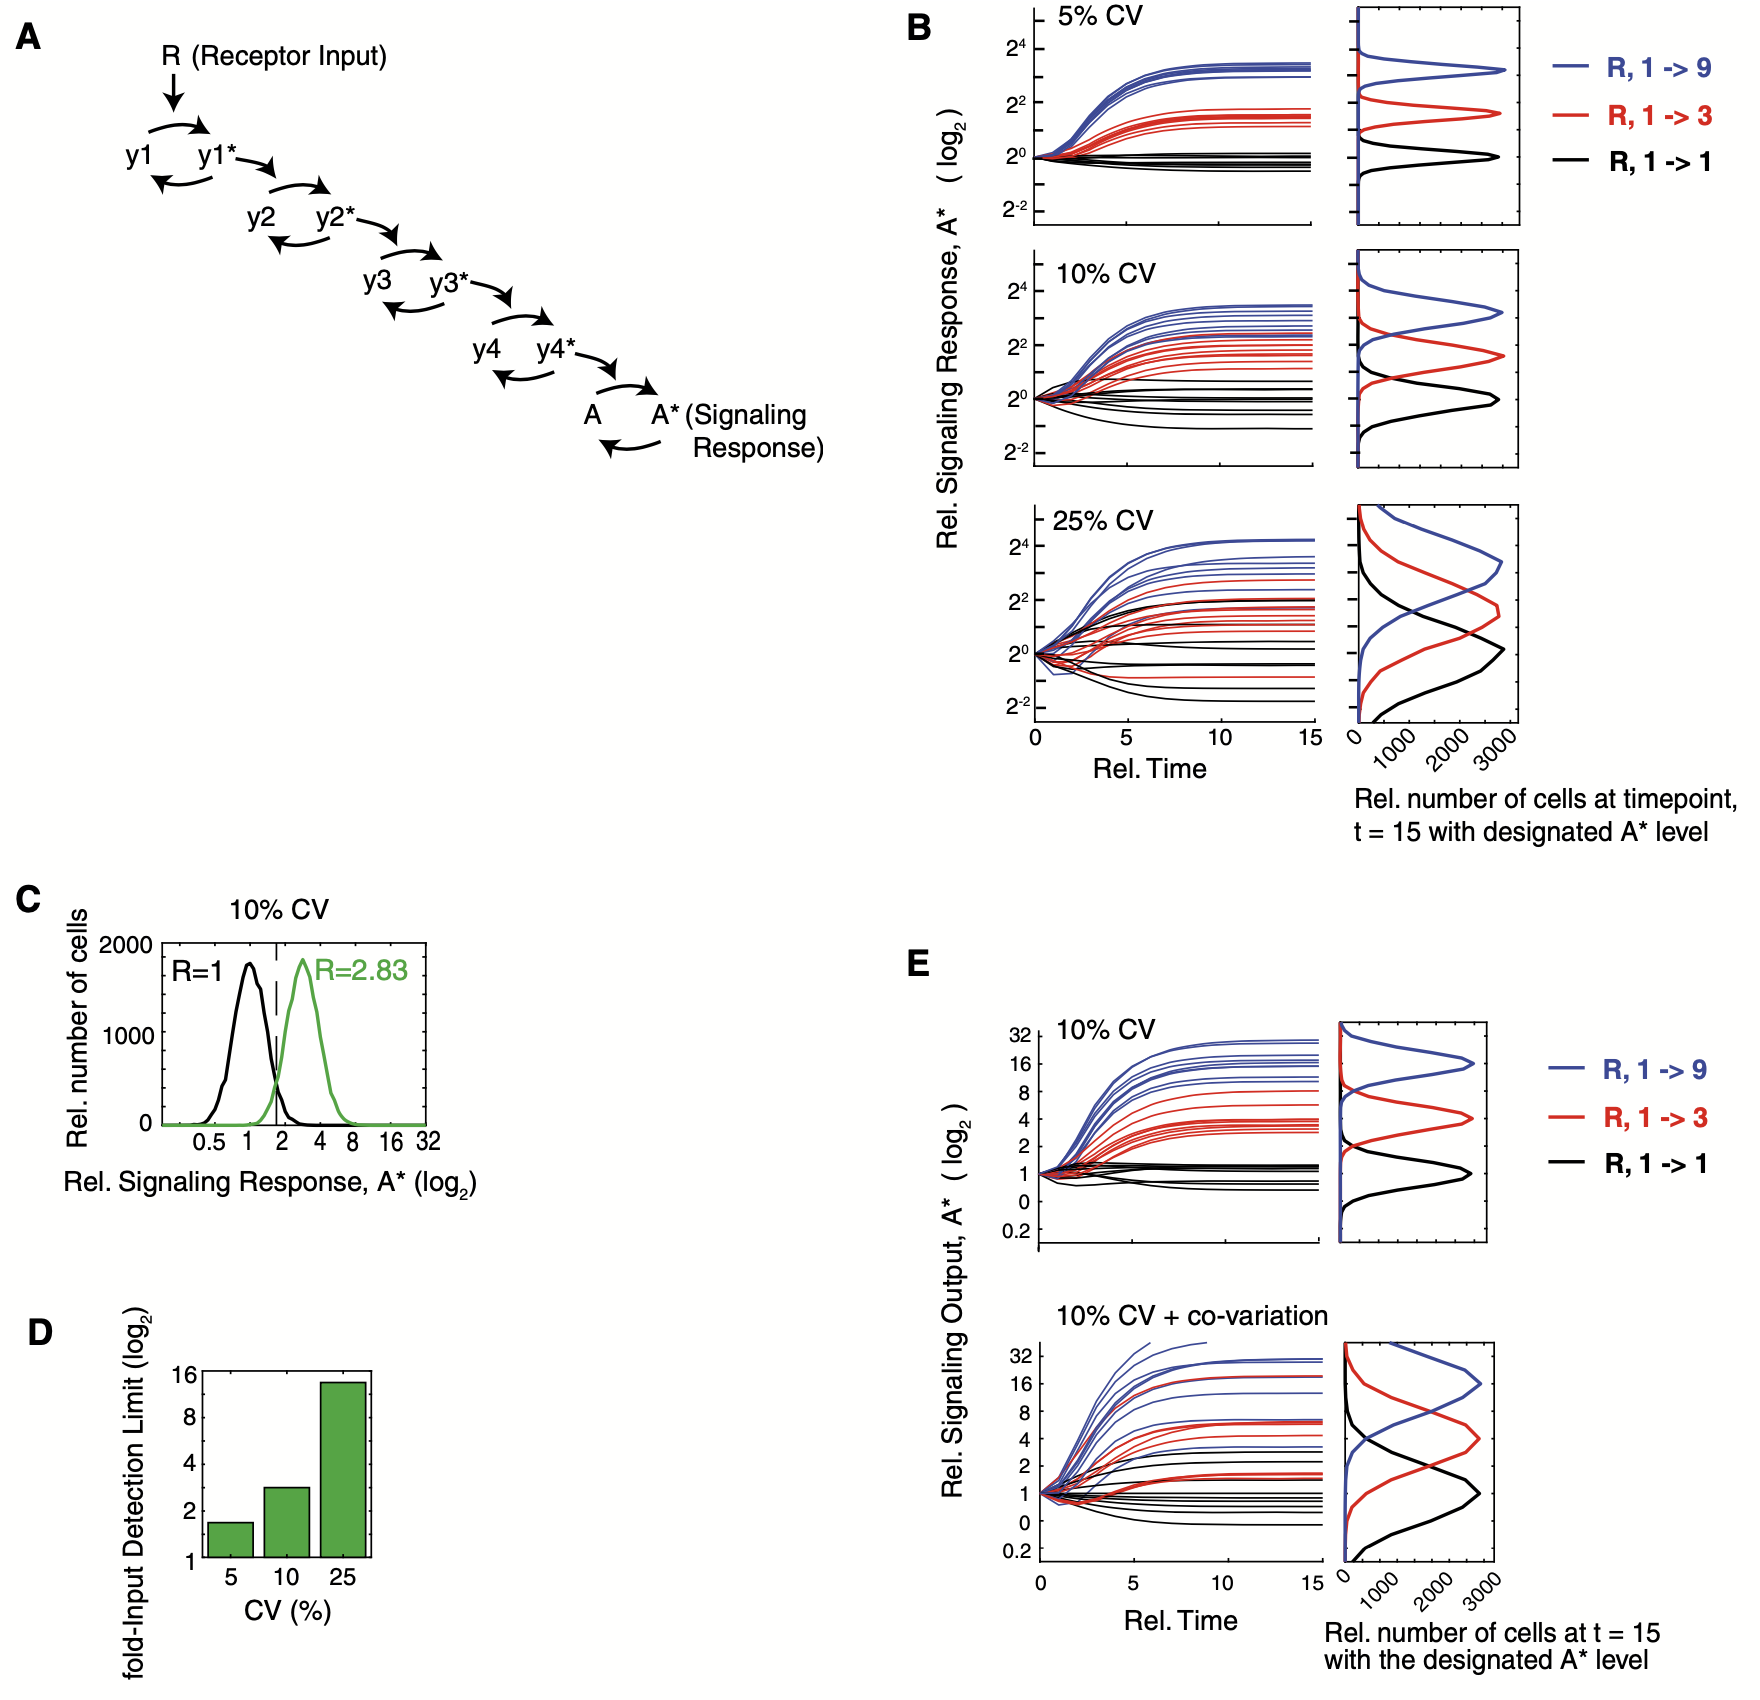
\includegraphics[width=14cm, keepaspectratio]{figs/paper1/fig1.png}
\caption[Short figure caption for List of Figures]{Long figure caption text that explains everything.}
\label{fig:paper1_fig1}
\end{figure}

There will be more text here.

More text here.

More text here.

More text here.

More text here.

More text here.

\subsection{Result 2}
We discovered something else. Here is a reference to Table \ref{tab:paper1_tab1}.

\renewcommand{\arraystretch}{2}  % make spacing nicer
\begin{table}[hbt!]
\centering
\begin{tabularx}{\textwidth}{c|c|c|c}  % 4 columns center-justified
   \textbf{Col 1} & \textbf{Col 2} & \textbf{Col 3} & \textbf{Col 4} \\
   \hline  % horizontal line
   Text in Row 1a & Text in Row 1b & Text in Row 1c & Lots of text in Row 1d \\
                  & Row 1.5b & Row 1.5c & Row 1.5d \\
   \hline
   Row 2a & Row 2b & Row 2c & Row 2d \\
   \hline
   Row 3a & Row 3b & Row 3c & Row 3d \\
\end{tabularx}
\caption[Short table caption for List of Tables]{Long table caption explaining everything.}
\label{tab:paper1_tab1}
\end{table}

More text here.

More text here.

More text here.

More text here.

\begin{sloppypar}
FixAwkwardSpacingWithSloppypar FixAwkwardSpacingWithSloppypar FixAwkwardSpacingWithSloppypar FixAwkwardSpacingWithSloppypar FixAwkwardSpacingWithSloppypar.
\end{sloppypar}

More text here.

More text here.

\section{Conclusions}
The end of the paper.

\chapter{Single-cell mass spectrometry identifies optimization of metabolic efficiency through low variance and high correlation of protein expression}
% Short title that appears in the header of pages within the chapter
\chaptermark{Module analysis of variance and correlation}

\begin{center}
Kyle M. Kovary, Zhibo Zhang, Mary N. Teruel
\end{center}

\vspace*{\fill}

%\begin{flushleft}
%The writing in this chapter contributed to the following publication:
%\end{flushleft}
%\newline
%\newline
%\bibentry{Kovary2018}

\newpage

\section{Abstract}
Protein expression variation leads to phenotypic variance between cells which, for example, in cell signaling and differentiation decisions, can lead to differences in cell fate. Targeted assays have shown correlation in expression of proteins that are part of larger assemblies or regulatory modules. However, there has not been a direct measurement of correlation within and between all protein modules in a single cell. Here we measure variation and correlation of over 1000 proteins in individual cells using quantitative proteomics of individual Xenopus laevis eggs and found that proteins involved in the same metabolic module tend to have low levels of expression variance, as well as high correlation. Markedly, we also identified a meta-logic of correlation that reflects the connection between metabolic modules. Molecular modeling showed that low variance and high correlation within metabolic modules results in higher efficiency of metabolic pathways. Additionally, the meta-analysis shows that related metabolic modules such as oxidative phosphorylation and lipid metabolism have high levels of correlation with one another, likely further maximizing overall efficiency. Our study argues for a control principle whereby coordinated variance and correlation within and between metabolic modules helps cells to increase metabolic efficiency.

\section{Highlights}
\begin{itemize}
\item Carried out large-scale analysis of variation and correlation of protein expression in single cells
\item Found that metabolic pathways tend to have low variation and high co-variation of protein expression, which would allow cells to express proteins at their ideal stochiometric levels that would maximize pathway efficiency.
\item Strategy of correlated expression of proteins extends beyond just individual modules and functionally related modules have higher than expected correlations.
\end{itemize}

\section{Introduction}
It is well known that variation in protein expression in single cells is important for adding diversity to functions and fate in populations of genetically homogenous cells (Ahrends et al., 2014; Kovary et al., 2018; Spencer et al., 2009; Suderman et al., 2017).  For example, high amounts of variance can decrease the output of a metabolic pathway but can increase the population level control of a binary signaling pathway. 

However since it has become more and more apparent that the functional units in cells are not an individual protein, but rather groups of proteins working together (e.g. signaling pathways, metabolic pathways, and protein complexes), here referred to as modules, it is important to understand how variation in protein expression affects the cell on a modular level. Since there are multiple proteins in modules, it thus becomes important to understand not just the variation in expression of a single protein but how the variation in expression of individual proteins is correlated.

When quantifying correlation between proteins, it is important to take into account the state of the cell since cell states can result in artifactual protein correlation. For example, not taking into account cell size can lead to misleading measures of correlation since larger cells will on average be expressing more proteins than smaller cells. However, after accounting for cell states that are not of interest, the remaining correlation can be used to understand the regulation of protein within modules as well as related modules. This remaining covariation could be indicative of upstream signaling and regulatory process such as shared transcriptional regulation (Stewart-Ornstein et al., 2012), co-translation (Li et al., 2014; Shi et al., 2017), and co-degradation (Mcshane et al., 2016).

Though the collective noise of proteins expressed in modules is key to understanding cellular behavior, the ability to measure module noise is challenging. Part of the challenge is that such measurements require measuring the abundance of many proteins in the same single cell. In a study carried out in yeast, the expression of 743 GFP-tagged proteins versus 44 RFP-tagged proteins was measured. The correlation of the noise, or “noise regulons” were calculated, and the resulting analysis suggested that these noise regulons can be used to identify signaling modules (Stewart-Ornstein et al., 2012). In vertebrate cells, co-variation of tens of proteins have been measured indirectly using antibodies followed by imaging (Gut et al., 2018), flow cytometry (Gaudet et al., 2012), or Cytof mass cytometry (Bendall et al., 2011). Analysis of the single-cell proteome using mass spectrometry analysis is difficult due to the small size of typical cells and the relative low efficiently of peptide-detection, but emerging techniques have shown that it can be useful for tracking cell state changes over time (Budnik et al., 2018).  

Because of the importance of protein modules rather an individual protein as the functional unit in cells, we need a way to be able to measure protein variation and covariation within modules. Mass spectrometry has been a workhorse for proteomics studies, however given the potential for noise in small sample sizes, single cell mass spectrometry has been rarely used. Here we tested whether using Xenopus laevis eggs, a vertebrate single cell model with a several order magnitude larger size, would enable robust simultaneous measurements of variation and co-variation of proteins on a proteome-wide scale and could overcome the signal-to-noise limitations caused by low sample protein levels in individual mammalian cells. We prepared samples of Xenopus laevis eggs during their first cell cycle following previously published protocols (Kovary et al., 2018) and conducted shotgun proteomics analyses. With this data set we have been able to gain insights into the relationship between protein expression variance, coordinated protein expression, and module variance at a proteomic scale in single cells. We identified classes of proteins that include heteromeric complexes and metabolic pathways that are expressed in such a way that can allow modules that rely on stoichiometric expression to function at higher levels of efficiency. Through coordinated expression (correlation) of proteins in a module with low expression variance, cells can express proteins in given complex or pathway at more stable and stoichiometric levels. Seeing multiple examples of the low variation and high correlated modules suggests that this elegant balancing act may be a general control strategy that allows for finer control of metabolic throughput and controlling the number of potentially formed complexes by expressing constituents closer to their stoichiometrically ideal levels. Through network analysis we show that this strategy extends beyond individual modules and can be used between functionally related modules.

\section{Results}
\subsection{Single cell proteomics reveals global protein expression variability and coordinated expression between protein pairs.}

Multicomponent modules such as heteromeric protein complexes and metabolic and signaling pathways have certain tolerances for noise. Two components of the noise of modules are the expression variance of the individual proteins, as well as the correlation of expression between the proteins. These noise components can be combined using the variance sum law (Equation 1) to quantify the total variance of the module. This value has the potential to be misleading given that the same level of total variance can have vastly different values of variation and covariation (Fig 1A, orange lines). For example, a hypothetical module of two proteins could have a total variance level of 0.25 while the proteins in one scenario have variance and correlation values of 0.25 and 0, and another with variance and correlation values of 0.247 and 0.75 (Fig. 1A-B, blue and red respectively). Our previous work has shown that increased levels of correlation, while having a small impact on total variance, can have huge effects on signaling behavior between single cells (Kovary et al., 2018). In order to understand the impact of noise on modules, it is therefore very important to study not only the variance of protein expression but also the correlation. In order to study the levels of variance and correlation of modules at a large scale, the constituent proteins must be measured simultaneously in single cells.

In order to study the relationship between protein expression variance and correlation of cellular pathways and complexes at the proteome level, we used Xenopus laevis eggs as a single cell model for proteomics. We activated Xenopus laevis eggs with calcium ionophore to initiate the cell cycle. We collected 5 eggs at 5 time points (0, 20, 40, 60, and 80 minutes) across the first cell cycle during which the egg remained a single cell following established protocols (Tsai et al., 2014)  (Fig S1A). Individual eggs were mechanically lysed and centrifuged to deplete the yolk the proteins. The proteins were then digested into peptides, labeled using TMT isobaric tags, multiplexed, and analyzed using a shotgun mass spectrometry approach. The relative abundance of more than 1000 proteins in each egg was quantified. Expression of the measured proteins across the time course of the cell cycle showed no dynamic pattern, as demonstrated by a PCA analysis which showed no discernible clustering of the eggs on cell cycle time (Fig. S1B), in agreement with previous studies of Xenopus laevis eggs at this stage (Presler et al., 2017). This result supports the conclusion that the proteins included in our analysis are likely not regulated by cell cycle processes, consistent with previous results which showed that only classic cell cycle protein regulators such as Cyclin A had significant changes in abundance during the first cell cycle (Kovary et al., 2018).  We thus used all 25 eggs for the analysis without distinguishing timepoints in order to increase our statistical observations.

To determine the expression variability for the measured proteins between single cells, we calculated the coefficient of variation (CV) for each protein across all 25 samples and observed a wide range of variation (Fig. 1C), many of which are consistent with our previous study of variation using targeted mass spectrometry (Fig. SXX). An added benefit to measuring these proteins in parallel is that we are able to calculate coordinated expression of protein pairs at a single cell resolution. Using the Pearson correlation coefficient, we were able to determine the coordinated expression of nearly 2 million protein pairs (Fig. 1D). The distribution of correlation coefficients fit a normal distribution centered around 0, with the majority of protein pairs appearing to not show significant co-regulation (Fig. S2). However, there appeared to be a significant number of protein pairs containing high correlation coefficients, and a clustered heat map showed that many highly co-regulated pairs cluster together (Fig. 1D).

This method allowed us to simultaneously measure the variance of individual proteins as well as the correlation between all protein pairs in single cells (Fig. 1E).

\subsection{Modules have varying levels of expression variance and coordinated expression of proteins}

In order to measure the variability and coordinated expression of proteins within modules, we used the KEGG ID and GO Term databases to categorize proteins into 1112 modules. In order for a module to be included it needed at least 4 proteins that were measured in single cells from our dataset. In order to have a single numeric value capture the overall variance of each module, the average CV of all of the proteins within a module was calculated (Average CV of the Module) (Fig 2A). We also wanted to provide a metric for the internal consistency of the variance of the proteins within a given module. For example, the CVs of proteins in the ribosome module (orange bars, Fig. 2C) are consistently low, but the CVs of the proteins in the GTPase module (purple bars, Fig. 2C) are a mixture of high and low.  By calculating the standard deviation of the variances within each module, we can consider modules that have consistent low or high levels of variance (Internal Consistency, Fig. SXX). This was done for all measured modules, and the module variance across the dataset ranged from 8\% to 34\%, with a median around 15\%. Figure 2B highlights 10 modules that had variances from high and low regions of the distribution. 

Fig 2C shows the protein abundance distributions and their respective CV’s for 10 representative modules that span the distribution of module variance (Fig 2A). For each module, the expression distribution and coefficient of variation for each protein could be analyzed individually. Modules such as the ErbB signaling pathway, large ribosomal subunit, and pentose phosphate pathway consistently have proteins with lower variance relative to the other proteins measured in this dataset. In previous work we discussed the observation and implications of low expression variance in modules like the ERK pathway (Mapk1 and Map2k1 are represented here as part of the ErbB module). It is interesting that metabolic pathways that are important at this stage of development had proteins with CVs that are consistently lower than the median. Pyruvate kinase, and with it glycolysis, has been shown to be largely inactive (Dworkin and Dworkin-Rastl, 1989a) while inhibition of the pentose phosphate pathway will quickly induce apoptosis for Xenopus oocytes and eggs (Nutt et al., 2005). This is likely due to the fact that at this stage of development carbohydrates are largely consumed by the pentose phosphate pathway to produce NADPH, an important cofactor and reducing agent for anabolic processes such as nucleic acid production. Phospholipid metabolism is highly active in Xenopus oocytes and fertilized eggs, with the yolk containing a significant amount of fatty acids that can be used for energy, leaving carbohydrates for NADHP metabolism. Many proteins in the fatty acid degradation module showed lower than average CVs (Dworkin and Dworkin-Rastl, 1989b). The low variance of the pentose phosphate and fatty acid degradation modules led us to hypothesize that enzymes belonging to highly active modules may be regulated in such a way as to reduce variance to reduce potential metabolic bottlenecks (add citations).

In addition to module variance, we set out to measure the average correlation of proteins in each module (average module correlation). To do this the Pearson correlation coefficient between all protein pairs within the module was calculated (Fig. 3A-B). We observed a range of module coordinated expression ranging from -0.17 to 0.43, with a median around 0.01 (Fig 3B-C). The distribution of module coordinated expression was biased towards the positive range, with some being very positive. 

We observed that heteromeric protein complexes such as the large ribosomal subunit and nucleosome had consistently high levels of coordinated expression of member proteins. This observation is consistent with reports of stoichiometric translation of complex members (Li et al., 2014) as well as the degradation of un-complexed nascent proteins (Mcshane et al., 2016). Additionally, we observed high levels of coordinated expression in the pentose phosphate pathway module, with exception of the proteins Tktl2, a protein similar to Tkt which showed high levels of coordinated expression, and Dera, a protein that may not always be relevant to the function of this pathway. 

Again, we observed contrasts between the glycolysis module with the pentose phosphate and fatty acid degradation modules. While the glycolysis module showed inconsistent levels of coordinated expression, the other two active metabolic modules showed consistent high levels of coordinated expression. Mathematically, high levels of coordinated expression increases variation in a pathway. However, models of E. coli metabolic pathways have shown that it can increase growth rates (Labhsetwar et al., 2013). 

\subsection{Metabolic pathways express proteins with lower than average variance and higher than average correlation.}

It has been demonstrated our previous work and others that the levels of protein expression variance and correlation can have effect the behaviors or efficacy of signaling pathways (Kovary et al., 2018; Suderman et al., 2017). In this study we had a unique opportunity to look at the variance (Fig. 2A) and correlation (Fig. 3A) of protein expression at the module level. When these two parameters were plotted together, we saw that there was a population of modules that occupied the low variance and high correlation space (Fig. 4A). This was surprising to us since modeling our previous work showed that high variance and high correlation is optimal for controlling fractional responses of binary signaling pathways of a population of cells, while low variance and low correlation is optimal for analog signaling pathways. We had not considered what pathways might utilize a low variance and high correlation modality.

To identify what broader categories of modules were in this population we used CateGOrizer, a method of GO term classification (Hu et al., 2008). This allowed us to place the modules into broader categories to identify overrepresented categories in the low variance / high correlation quadrant. By comparing this population of modules to the remaining population, we saw that this region was greatly enriched for metabolic pathways (Fig. 4B). 

Metabolic pathways have properties that make them distinct from signaling pathways, including the fact that they can consume, produce, and compete for molecules used in other metabolic pathways. In order to study what advantages this strategy of low variance and high correlation may have for metabolic pathways, we constructed a simple branched metabolic model where a substrate is converted into a product via two enzymes with identical reaction rates that compete with another pathway for the intermediate molecule (Fig. 4C). Using this simple ODE model, we were able to vary the expression variance and correlation of the two enzymes and randomly sampled 1000 cells from these populations (Fig. 4D).

To quantify the efficiency of the pathway, we defined efficiency as the concentration of product produced relative to the sum of the concentrations of the two enzymes. We found that both decreasing the variance of the enzymes as well as increasing the correlation of two enzymes increased efficiency, with noticeable synergistic effects (Fig. 4E). This result becomes intuitive after considering that decreasing variance and increasing correlation results in proteins being produced closer to their ideal stoichiometric levels. In the case of this idealized model, the optimal stoichiometric levels are 1:1, but this strategy could optimize expression for pathways with any stoichiometric requirements. By approaching this optimal ratio, the observed pathway was able to consume the intermediate at a faster rate, allowing it to better compete with the alternative branched pathway and produce the observed product.

\subsection{Network analysis of modules shows coordinated expression of lipid, amino acid, and mitochondrial proteins}

In early development of Xenopus embryos, yolk protein and lipids are a key source of nutrition and energy (Jorgensen et al., 2009). Additionally glycolysis, a principal energetic pathway feeding into the citric acid cycle, has been shown to be inactive at this stage of development (Dworkin and Dworkin-Rastl, 1989a). Since module level coordinated expression of metabolic pathways appeared to increase efficiency, we wondered if this optimization could be observed between modules (e.g. lipid metabolism and the citric acid cycle).

To illustrate the idea of between module correlations, Figures 5A and 5B show correlation matrices of the mitochondrial protein complex with superoxide dismutase (SOD) activity and mitotic nuclear division modules. The mitochondrial proteins correlate strongly with the SOD enzymes, and therefore there is a lack of clustering between these two modules (Fig. 5A). This relationship is intuitive given the role SOD enzymes play in reducing reactive oxygen species (ROS) produced by mitochondria through the TCA cycle. If more active mitochondrial proteins are created, there could be a proportional increase in ROS. By coordinating the expression of these proteins with SOD enzymes, cells would be better able at reducing ROS levels.

The negative correlations between the mitochondrial protein complex and mitotic nuclear division modules results in strong clustering of these two modules individually in the correlation matrix heatmap (Fig. 5B). This striking negative relationship is in line with the fact that at the onset of mitosis, mitochondria undergo fission before being reassembled later in the cell cycle (Lu et al., 2006). Mitochondrial fusion has been linked to increased levels of oxidative phosphorylation (Yao et al., 2019), and there is evidence that oxidative phosphorylation activity decreases entering mitosis (Kang et al., 2019). This negative coordinated expression between mitosis and mitochondrial protein complex modules could be due to decreased oxidative phosphorylation activity due to mitochondrial fission when cells enters mitosis.

These two targeted examples give credence to the concept of measuring between module correlations and led us to develop a method to identify links between modules at a larger scale. We conceptualized a bait-prey framework that considered the pairwise relationship between all measured modules that had no overlapping proteins. We conducted a statistical test where new pairwise correlations of proteins between the modules was assumed to be zero and compared this to the measured correlation coefficients (Fig 5C). This assumption was based on the distribution of correlation coefficients between all measured protein pairs, which was centered around zero (Fig. S1). A p-value was calculated between the observed and null distributions of correlation coefficients that was corrected for multiple hypothesis testing using a false discovery rate method. Interactions between modules were considered to be significant if the corrected p-value was less than 0.05. In order to classify the between module interactions as positive or negative, we compared the measured module level correlation to the null hypothesis, where a greater than null value was classified as positive, and a less than null value was classified as negative. This analysis can be graphically represented as a volcano plot for each module individually (example in Fig. 5D) or as a network of all modules together where each module is a node and the positive or negative interactions between each module are edges (Figs. 5E-F).

The interaction network for the oxidative phosphorylation module is highlighted in Figure 5D. Each point represents a test between the oxidative phosphorylation module with all other measured modules. The points highlighted in orange are positive interaction modules, and the points highlighted in blue are negative interaction modules. Interestingly, lipid and amino acid degradation modules were found to have positive interactions with oxidative phosphorylation, whereas carbohydrate and glycolysis modules were found to have negative interactions with oxidative phosphorylation. This is strong evidence that correlated expression of proteins extends beyond individual modules and in fact can span between connected modules. Given that yolk is a major source of energy and resources that is consumed over the course of embryogenesis, the coordinated expression of metabolic pathways that metabolize lipids and amino acids into molecules that are fed into the citric acid cycle with the members of that cycle would be a powerful strategy to increase metabolic efficiency (Fig. 4E). Recent work has shown that pathway specific mRNAs can be co-translated (Shi et al., 2017), and that nuclear-encoded mRNAs can be localized to the mitochondria to be translated (Tsuboi et al., 2020), two potential strategies that may be utilized here given that lipid and amino acid degradation can happen within mitochondria.

The relationships between all of these modules can be visually represented as a network graph (Figs. 5E-F). Each of these networks is comprised of several neighborhoods, some with connections between them and others that are isolated. For instance, the positive relationship network contained one neighborhood (Fig. 5 D, orange) that was comprised primarily of protein translation machinery and mitochondrial modules, suggesting that there is a strong positive relationship between ribosomal protein expression and mitochondria at this stage of development. This neighborhood is closely related to a second (Fig. 5D, green) that contained oxidative phosphorylation modules that were tightly linked with various metabolic pathways including lipid metabolism and amino acid degradation pathways.  

The negative relationship network provides additional strength to the previous insights based on the positive relationship network (Fig. 5E). Here we see negative correlations between oxidative phosphorylation and carbohydrate metabolic processes. As stated earlier, much of carbohydrate metabolism is focused on production of NADPH through the pentose phosphate pathway rather than on the production of ATP through oxidative phosphorylation in the mitochondria. This provides further evidence that measuring correlation of protein expression in single cells can elucidate metabolic strategies of cells.

\section{Materials and Methods} \label{Materials and Methods}

\subsection{Collection and activation of \emph{Xenopus laevis} eggs.}

All of the animal protocols used in this manuscript were approved by the Stanford University Administrative Panel on Laboratory Animal Care. Xenopus egg extracts were prepared as previously described (Kovary et al., 2018), Briefly, to induce egg laying, female Xenopus laevis were injected with human chorionic gonadotropin injection the night before each experiment. To collect the eggs, the frogs were subjected to pelvic massage, and the eggs were collected in 1X Marc’s Modified Ringer’s (MMR) buffer (0.1 M NaCl, 2 mM KCl, 1 mM MgCl2, 2 mM CaCl2, 5 mM HEPES, pH 7.8). To remove the jelly coat from the eggs, they were placed in a solution of 2\% cysteine in 1× MMR buffer for 4 min and gently agitated, after which they were washed four times with 1× MMR buffer. To activate the cell cycle, eggs were placed in a solution of 0.5 μg/ml of calcium ionophore A23187 (Sigma) and 1X MMR buffer for 3 min, after which they were washed four times with 1× MMR buffer. Single eggs were collected at their respective time-points and placed into 600$\mu l$ tubes and snap frozen in liquid nitrogen before being stored at $-80$\si{\degree}C.

\subsection{Sample preparation for mass spectrometry}

Single eggs were lysed mechanically by pipetting the egg in 100$\mu l$ of lysis buffer (100 mM NaCl, 25 mM Tris pH 8.2, Complete EDTA-free protease inhibitor cocktail (Sigma). The lysate was then placed in a 400$\mu l$ natural polyethylene micro-centrifuge tube (E&K Scientific #485050) and spun at 15,000 g in a right-angle centrifuge (Beckman Microfuge E) at $4$\si{\degree}C for 5 min. The lipid layer was removed by using a razor blade to cut the tube off just beneath it, and the cytoplasmic fraction was pipetted into a 1.5-ml protein LoBind tube (Fisher Scientific 13-698-794), being careful to leave the yolk behind. To precipitate the proteins from the cytoplasmic fraction, 1 ml of ice-cold acetone was added to each sample and placed at $-20$\si{\degree}C overnight. To collect precipitated proteins, the samples were centrifuged at 18,000 g for 20 min at $4$\si{\degree}C. Acetone was decanted, and the protein pellets were resolubilized in 25$\mu l$ of 8 M urea. To fully solubilize the protein pellet, the samples were placed in a shaker for 1 h at room temperature. The samples were then diluted to 2 M urea with 50 mM ammonium bicarbonate to a 100μL volume, after which protein concentration was measured in duplicate with a BCA assay by taking two 10μL aliquots of each sample. The proteins in the remaining 80μL of sample volume were reduced with 10 mM TCEP and incubated for 30 min at $37$\si{\degree}C, then alkylated with 15 mM iodoacetamide and incubated in the dark at room temperature.

Next, the samples were diluted to 1 M urea with 50 mM ammonium bicarbonate. Trypsin (Promega #V5113) was then added at a ratio of 10ng trypsin per 1ug protein (no < 500 ng was added to a sample). The trypsin digestion was carried out at $37$\si{\degree}C for 12–16 h. To stop the trypsin, formic acid (Fisher A117-50) was added at a ratio of 3μl per 100μl of sample to bring the pH down to < 3.

Peptides were cleaned up using an Oasis HLB uElution plate (Waters), equilibrated, and washed with 0.04\% trifluoroacetic acid in water, and eluted in 80\% acetonitrile with 0.2\% formic acid. All solutions used are HPLC grade. Samples were then lyophilized. To remove any variance produced by phosphorylated peptides, the samples were phosphatase-treated. Peptides were resolubilized in 50$\mu l$ of 1X NEBuffer 3 (no BSA), and calf intestinal alkaline phosphatase (NEB M0290S) was added at a ratio 0.25 units per lg of peptide and incubated for 1 h at $37$\si{\degree}C. The peptides were cleaned up again according to steps described above.
Samples were then labeled with 6-plex Thermo Scientific Tandem Mass Tag (TMT) Reagents, using instructions provided by the manufacturer. The 25 samples were divided into 5 groups of 5 and pooled together with a master reference sample to create 6-plexed samples. Peptides cleaned up and resolubilized in 2\% acetonitrile and 0.1\% formic acid before MS analysis.

\subsection{Mass spectrometry data collection and analysis}

Peptide identification of each digestion mixture was performed by microcapillary reverse-phase HPLC nanoelectrospray tandem mass spectrometry (mLC-MS/MS) on an LTQ-Orbitrap Velos. The Orbitrap repetitively surveyed a mass/charge (m/z) range from 395 to 1,600, while data-dependent MS/MS spectra on the 20 most abundant ions in each survey scan were acquired in the linear ion trap. MS/MS spectra were acquired with a relative collision energy of 30\%, an isolation width of 2.5 Da and dynamic exclusion of recurring ions for 60 s. Preliminary sequencing of peptides was facilitated with the SEQUEST algorithm with a mass tolerance of 30 ppm against a species-specific (mouse or human) subset of the UniProt Knowledgebase. With a custom version of the Harvard Proteomics Browser Suite (Thermo Fisher Scientific), peptide spectrum matches (PSMs) were accepted with mass error <2.5 ppm and score thresholds to attain an estimated false discovery rate (FDR) of <1\% using a reverse-decoy database strategy.

\subsection{Data processing}

To minimize the effects of non-biological variance, a correction factor was used to correct for these biases. First, each peptide in each run was normalized its corresponding master reference channel (equal parts of all 25 eggs) after which peptides were grouped by their master Uniprot accession number and the average normalized intensity was calculate to represent the relative protein abundance. Proteins were then re-normalized by the mean protein value across all cells and then by the mean protein value within each cell. Missing protein levels were imputed using the k-nearest neighbors algorithm, with k being set to 3 and the similarity measure for distance the Gower’s distance between the proteome vectors.

\subsection{Statistical analysis of proteins}

To estimate the variability of expression of each protein between single cells, we calculated the coefficient of variance (CV), a unitless metric defined as the standard deviation divided by the arithmetic mean. This was done on non-transformed data since CV as defined above is would result in incorrect CVs (Canchola, 2017). To estimate the coordinated expression of each protein measured we calculated the Pearson’s correlation coefficient for each pair of proteins after Log2 transforming them in order to reduce the weight of potential outliers and to balance the influence of values below and above 1.

\subsection{Module analysis}

Proteins were grouped together into modules using GO term and KEGG pathway annotations. GO terms and KEGG pathways along with their associated proteins were retrieved using the R package org.Xl.eg.db (Carlson, 2020). In order to estimate module level variance, the CV values of all of the proteins associated with each module were aggregated and the arithmetic mean was calculated and used to represent module level variance. A similar approach was used to estimating module level coordinated expression. The arithmetic mean was calculated for the lower triangular matrix of the pairwise correlation matrix calculated for all protein pairs associated with each module and was used to represent module level coordinated expression.

In order to identify between module relationships, we considered all pairwise combinations of modules with zero overlapping proteins. To test whether combining the two modules resulted in a higher or lower than expected combined module level coordinated expression we constructed a null hypothesis where all new pairwise relationships between the two modules were assumed to be zero (no relationship). This distribution of correlation coefficients was compared to the true distribution. When the FDR corrected p-value, calculated through a Student’s t-test, was less than 0.05 then the pairwise relationship between the modules was classified as significant. We then measured if the arithmetic mean of the combined distribution of correlation coefficients was higher or lower than the null distribution to classify the relationship as positive or negative.

\subsection{GO-slim analysis}

Modules that had variances less than the population mean and correlations greater than the population mean were submitted to CateGOrizer separately from the rest of the population. The number of GO-terms assigned to each category from CateGOrizer was returned from the analysis. The counts of GO-terms assigned to each category was normalized to the total number of analyzed GO-terms such that all of the categories added up to 100\%.

\subsection{Metabolic Model}


\section{Figures}
% Figure 1
\begin{figure}[hbt!]
\centering
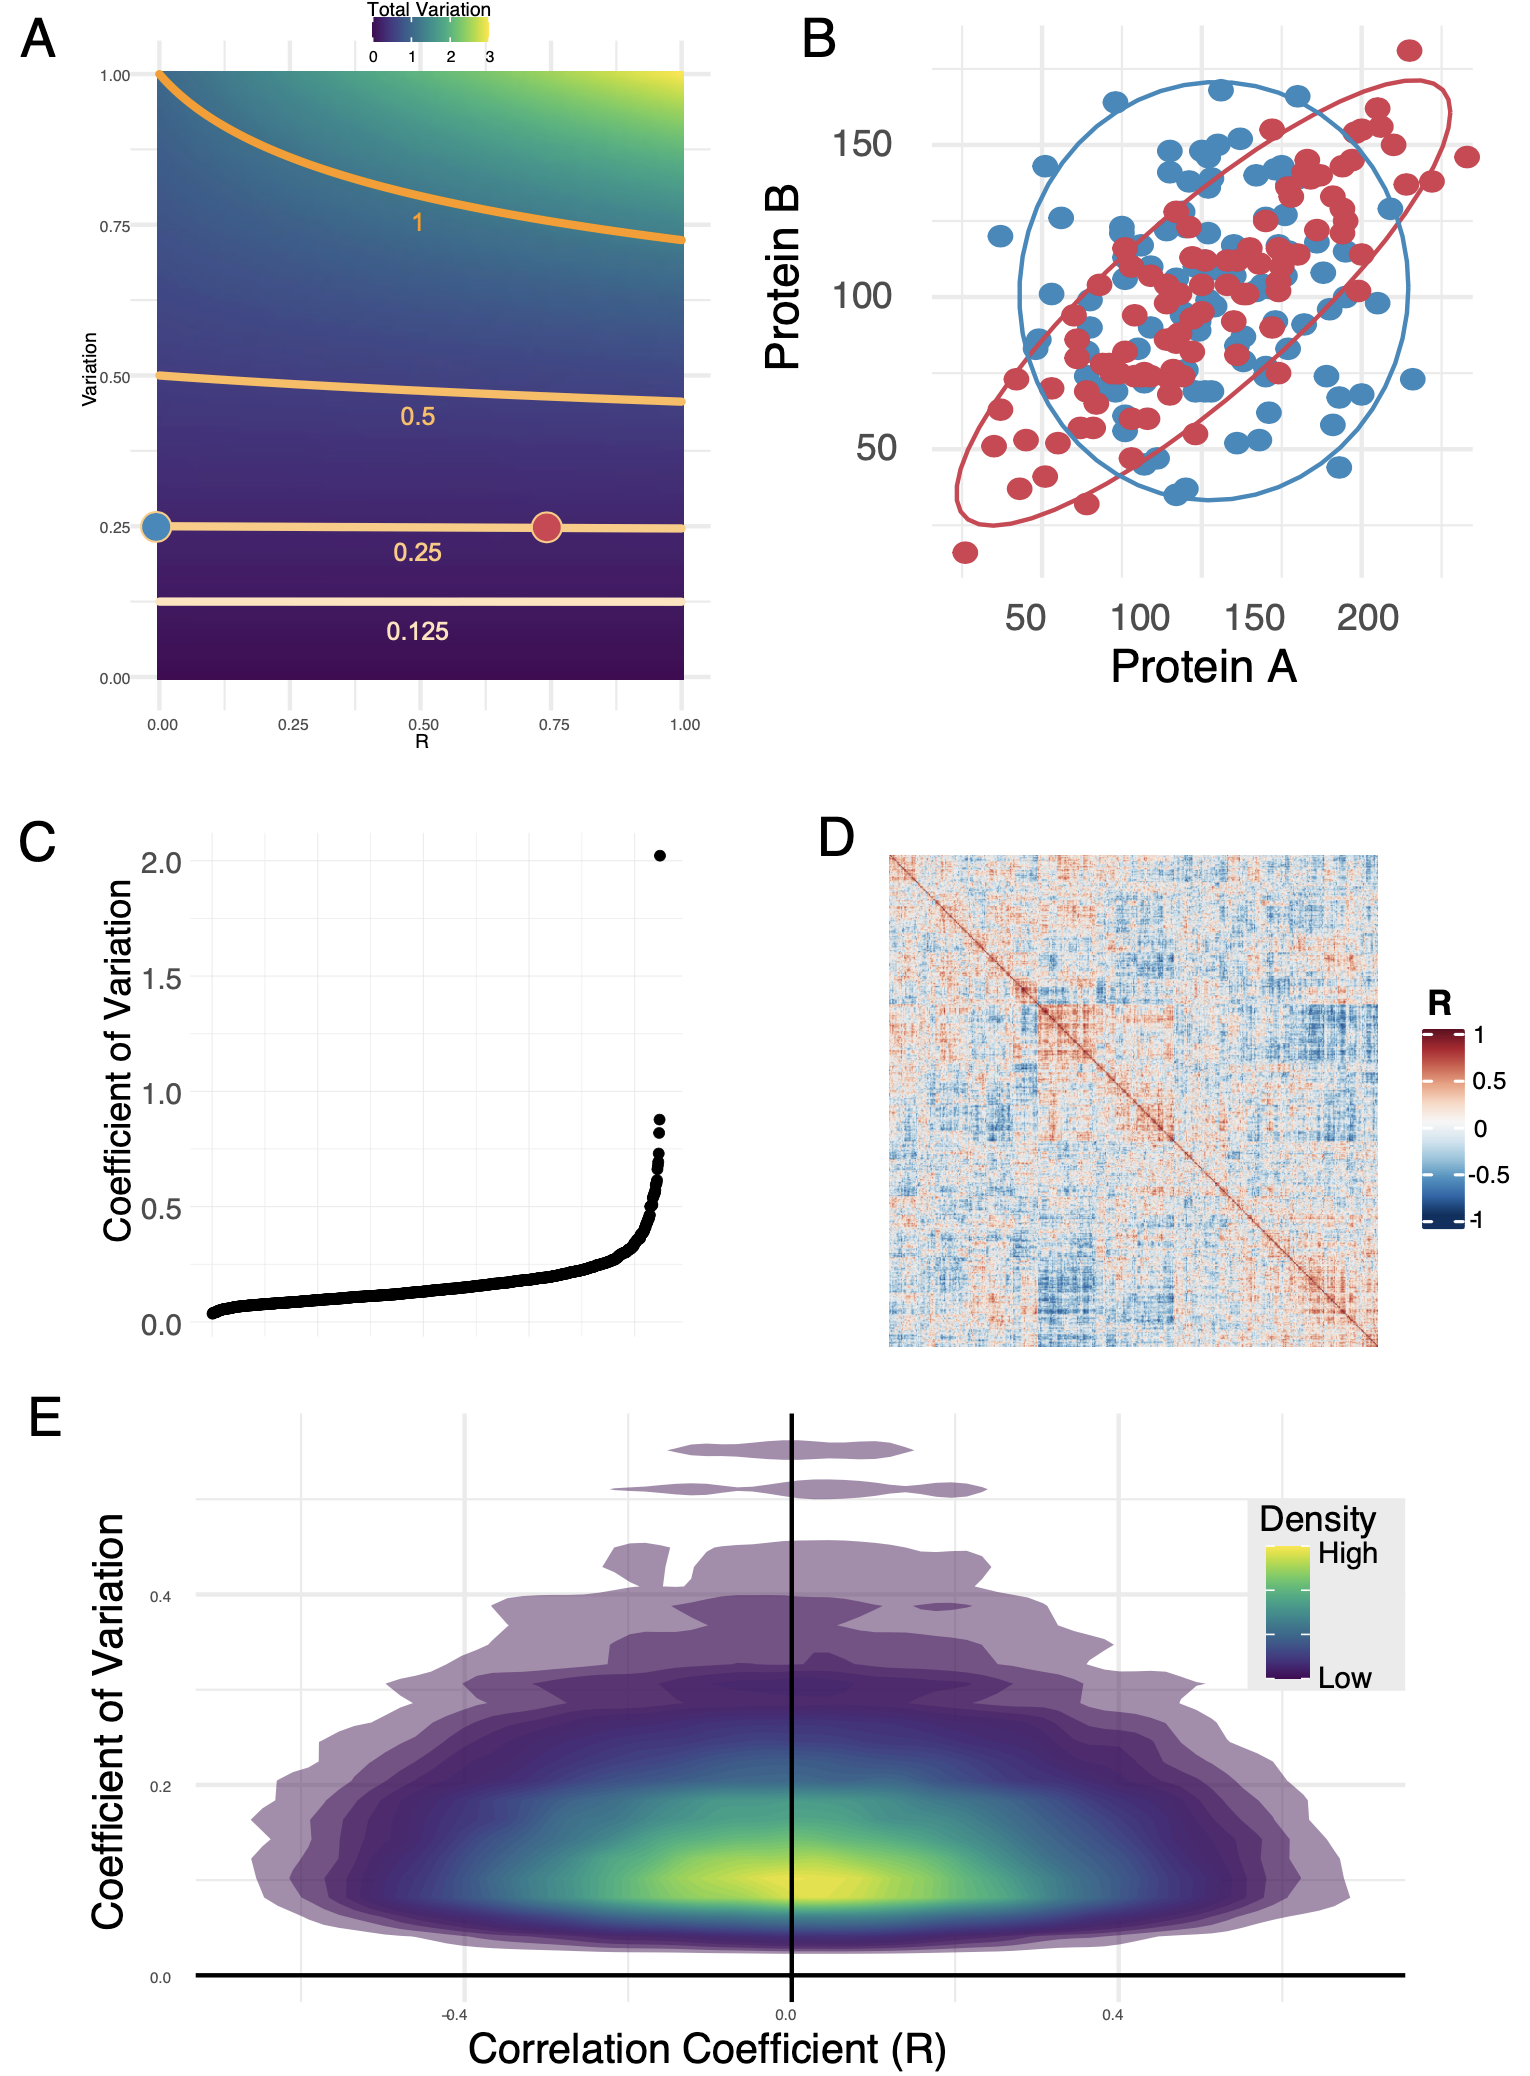
\includegraphics[width=12cm, keepaspectratio]{figs/paper2/fig1.png}
\caption{Single cell proteomics reveals global protein expression variability and coordinated expression between protein pairs.}
\caption*{\textbf{(A)} Heatmap of total variation (Equation 1) in relationship to correlation coefficient (x-axis) and variation (y-axis). Orange lines represent specific regions of equal total variance, and blue and red points represent the region where the distributions in (B) come from. \textbf{(B)} Pairwise plot of simulated distributions of proteins of equal variance. Though the protein distributions have the same total variance and similar variance, the correlated expression of the proteins are very different, which can have profound impacts on module function. \textbf{(C)} Ranked plot of the calculated coefficient of variation of each of the proteins quantified in single cells. \textbf{(D)} Heatmap of the correlation coefficients between all measured protein pairs. \textbf{(E)} Pairwise plot of all measured protein variances and covariances, colored by density.}
\label{fig:paper2_fig1}
\end{figure}

% Figure 2
\begin{figure}[hbt!]
\centering
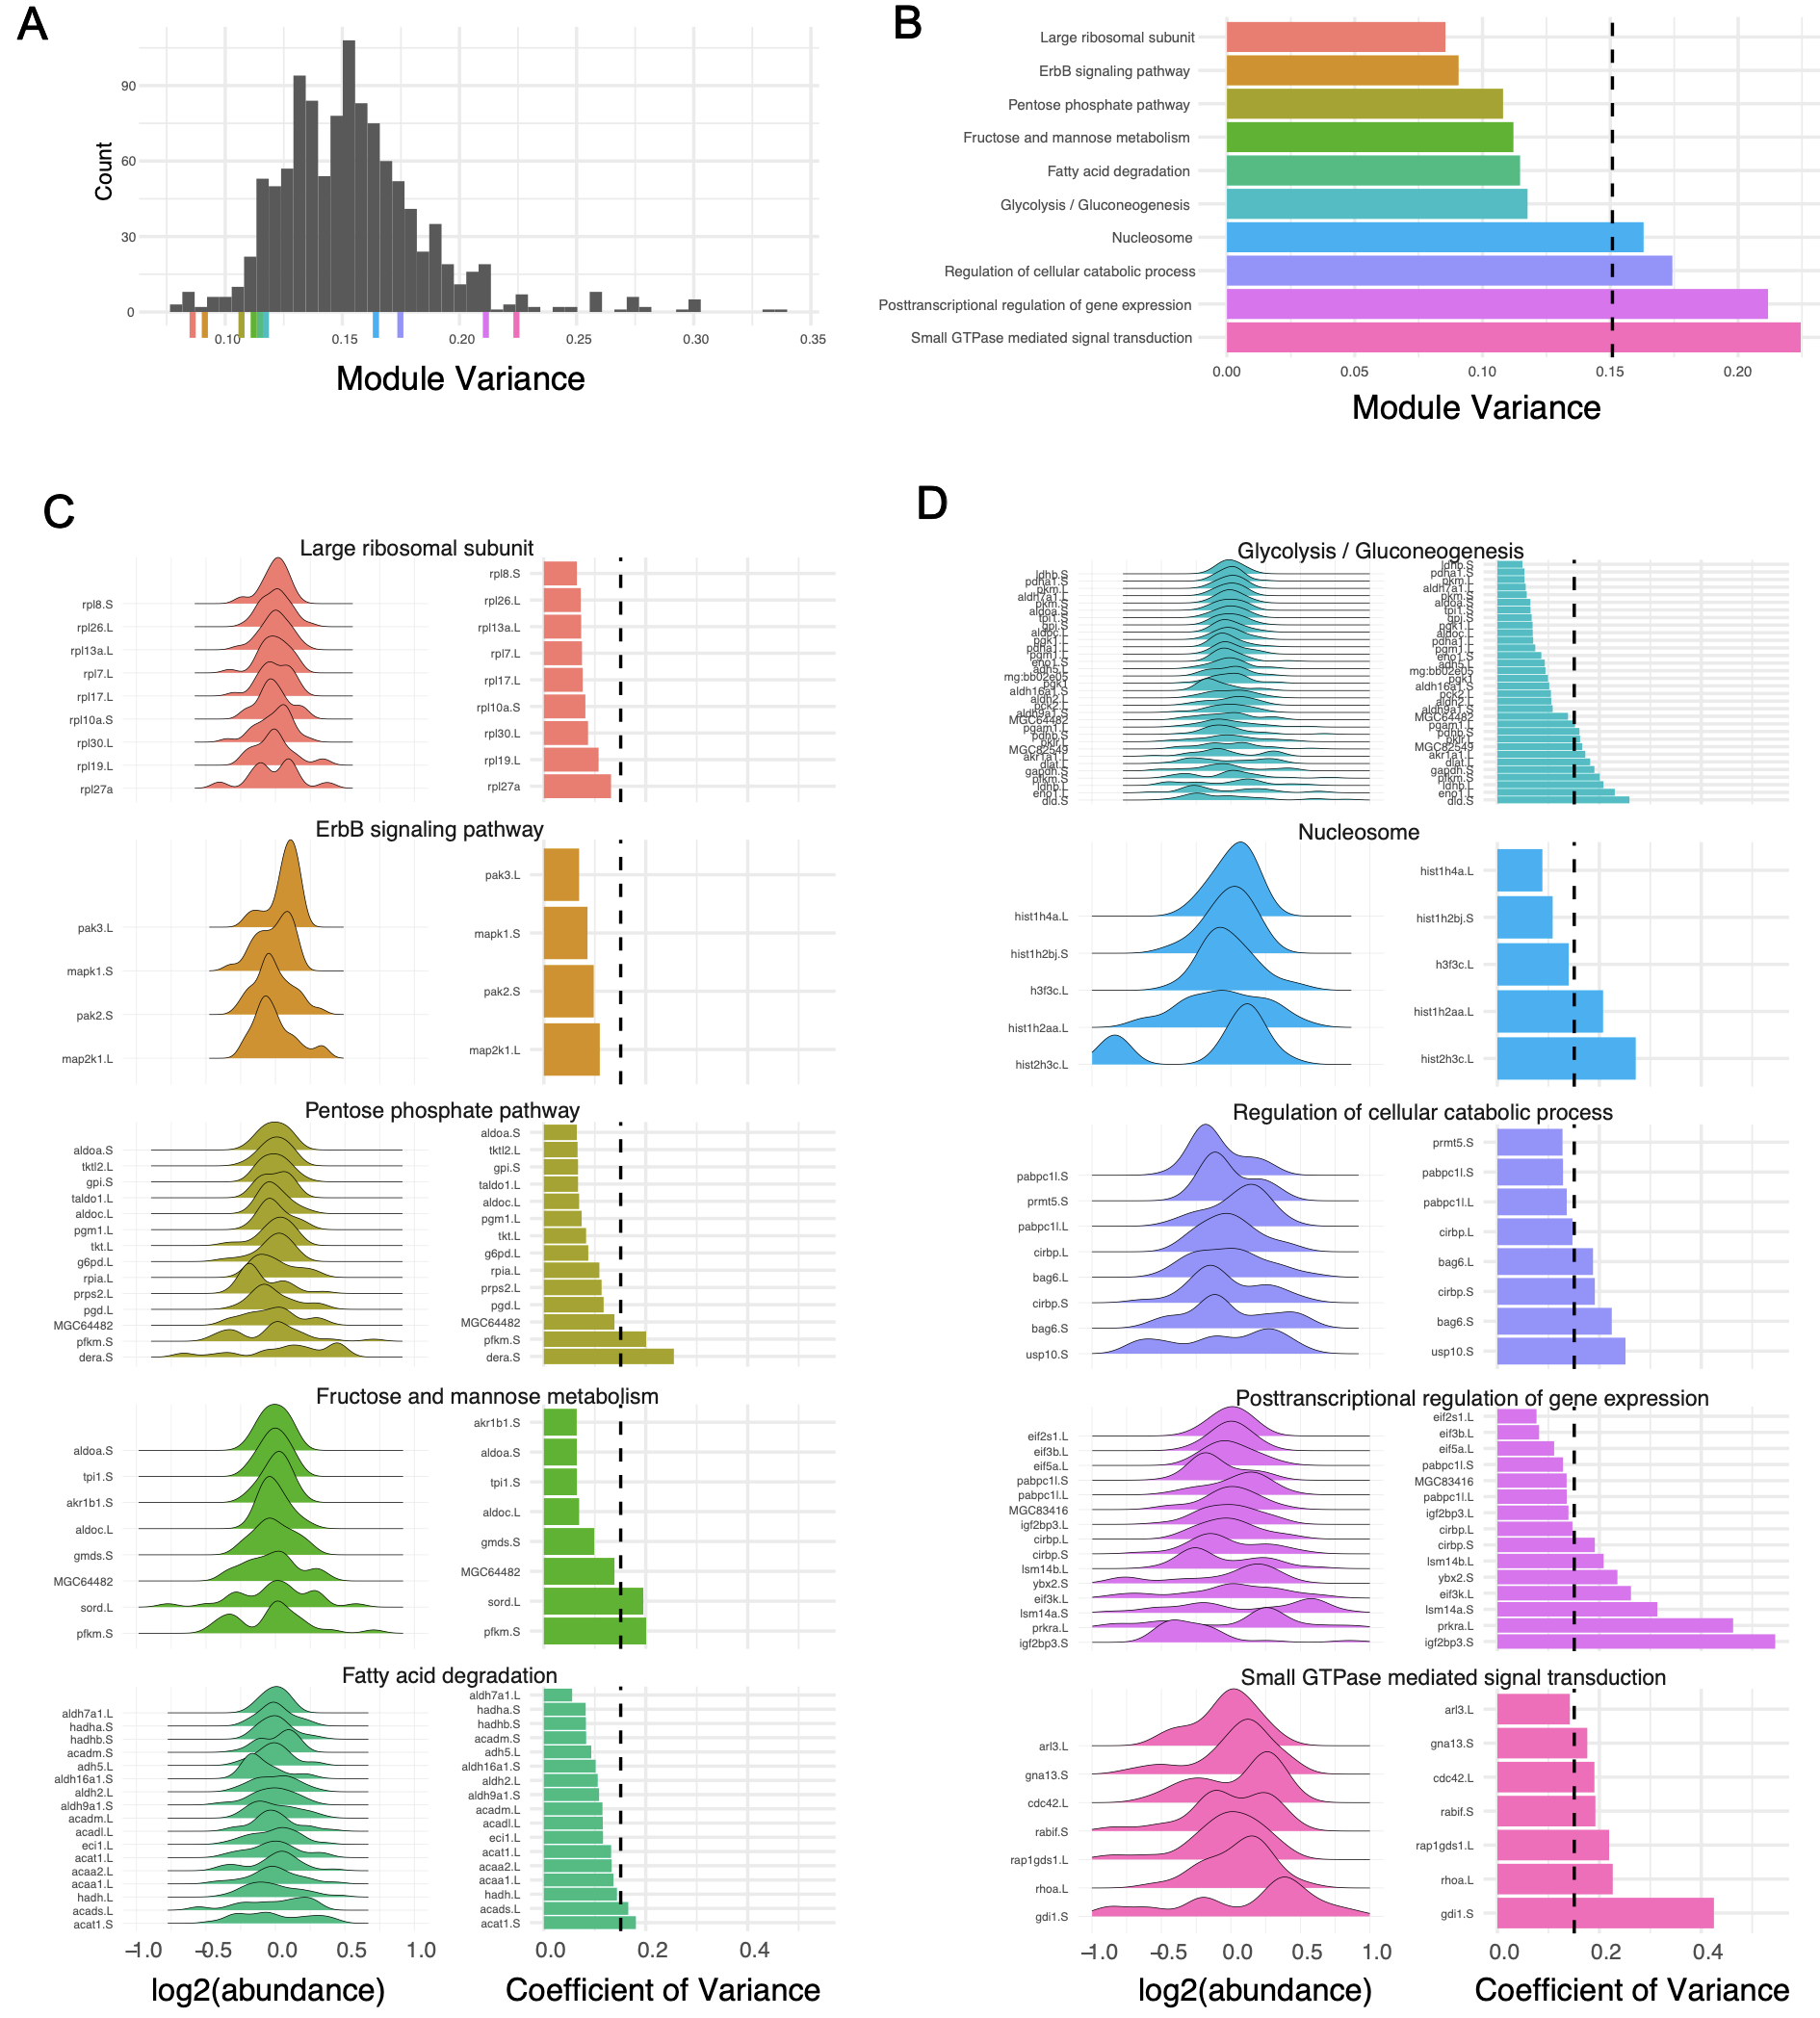
\includegraphics[width=15cm, keepaspectratio]{figs/paper2/fig2.png}
\caption{KEGG pathways and GO Terms can be used to group proteins together to identify modules that on average maintain low and high levels of expression variation.}
\caption*{\textbf{(A)} Density plots of the proteins assigned to each of the four modules represent the variation of expression. \textbf{(B)} Bar plots the coefficient of variation calculated for each protein. The dashed line represents the median coefficient of variation of all measured proteins. \textbf{(C)} Histogram of the average module variance of all modules analyzed in this dataset (1112). The module variance of each of the modules shown in A and B are colored below the plot.}
\label{fig:paper2_fig2}
\end{figure}

% Figure 3
\begin{figure}[hbt!]
\centering
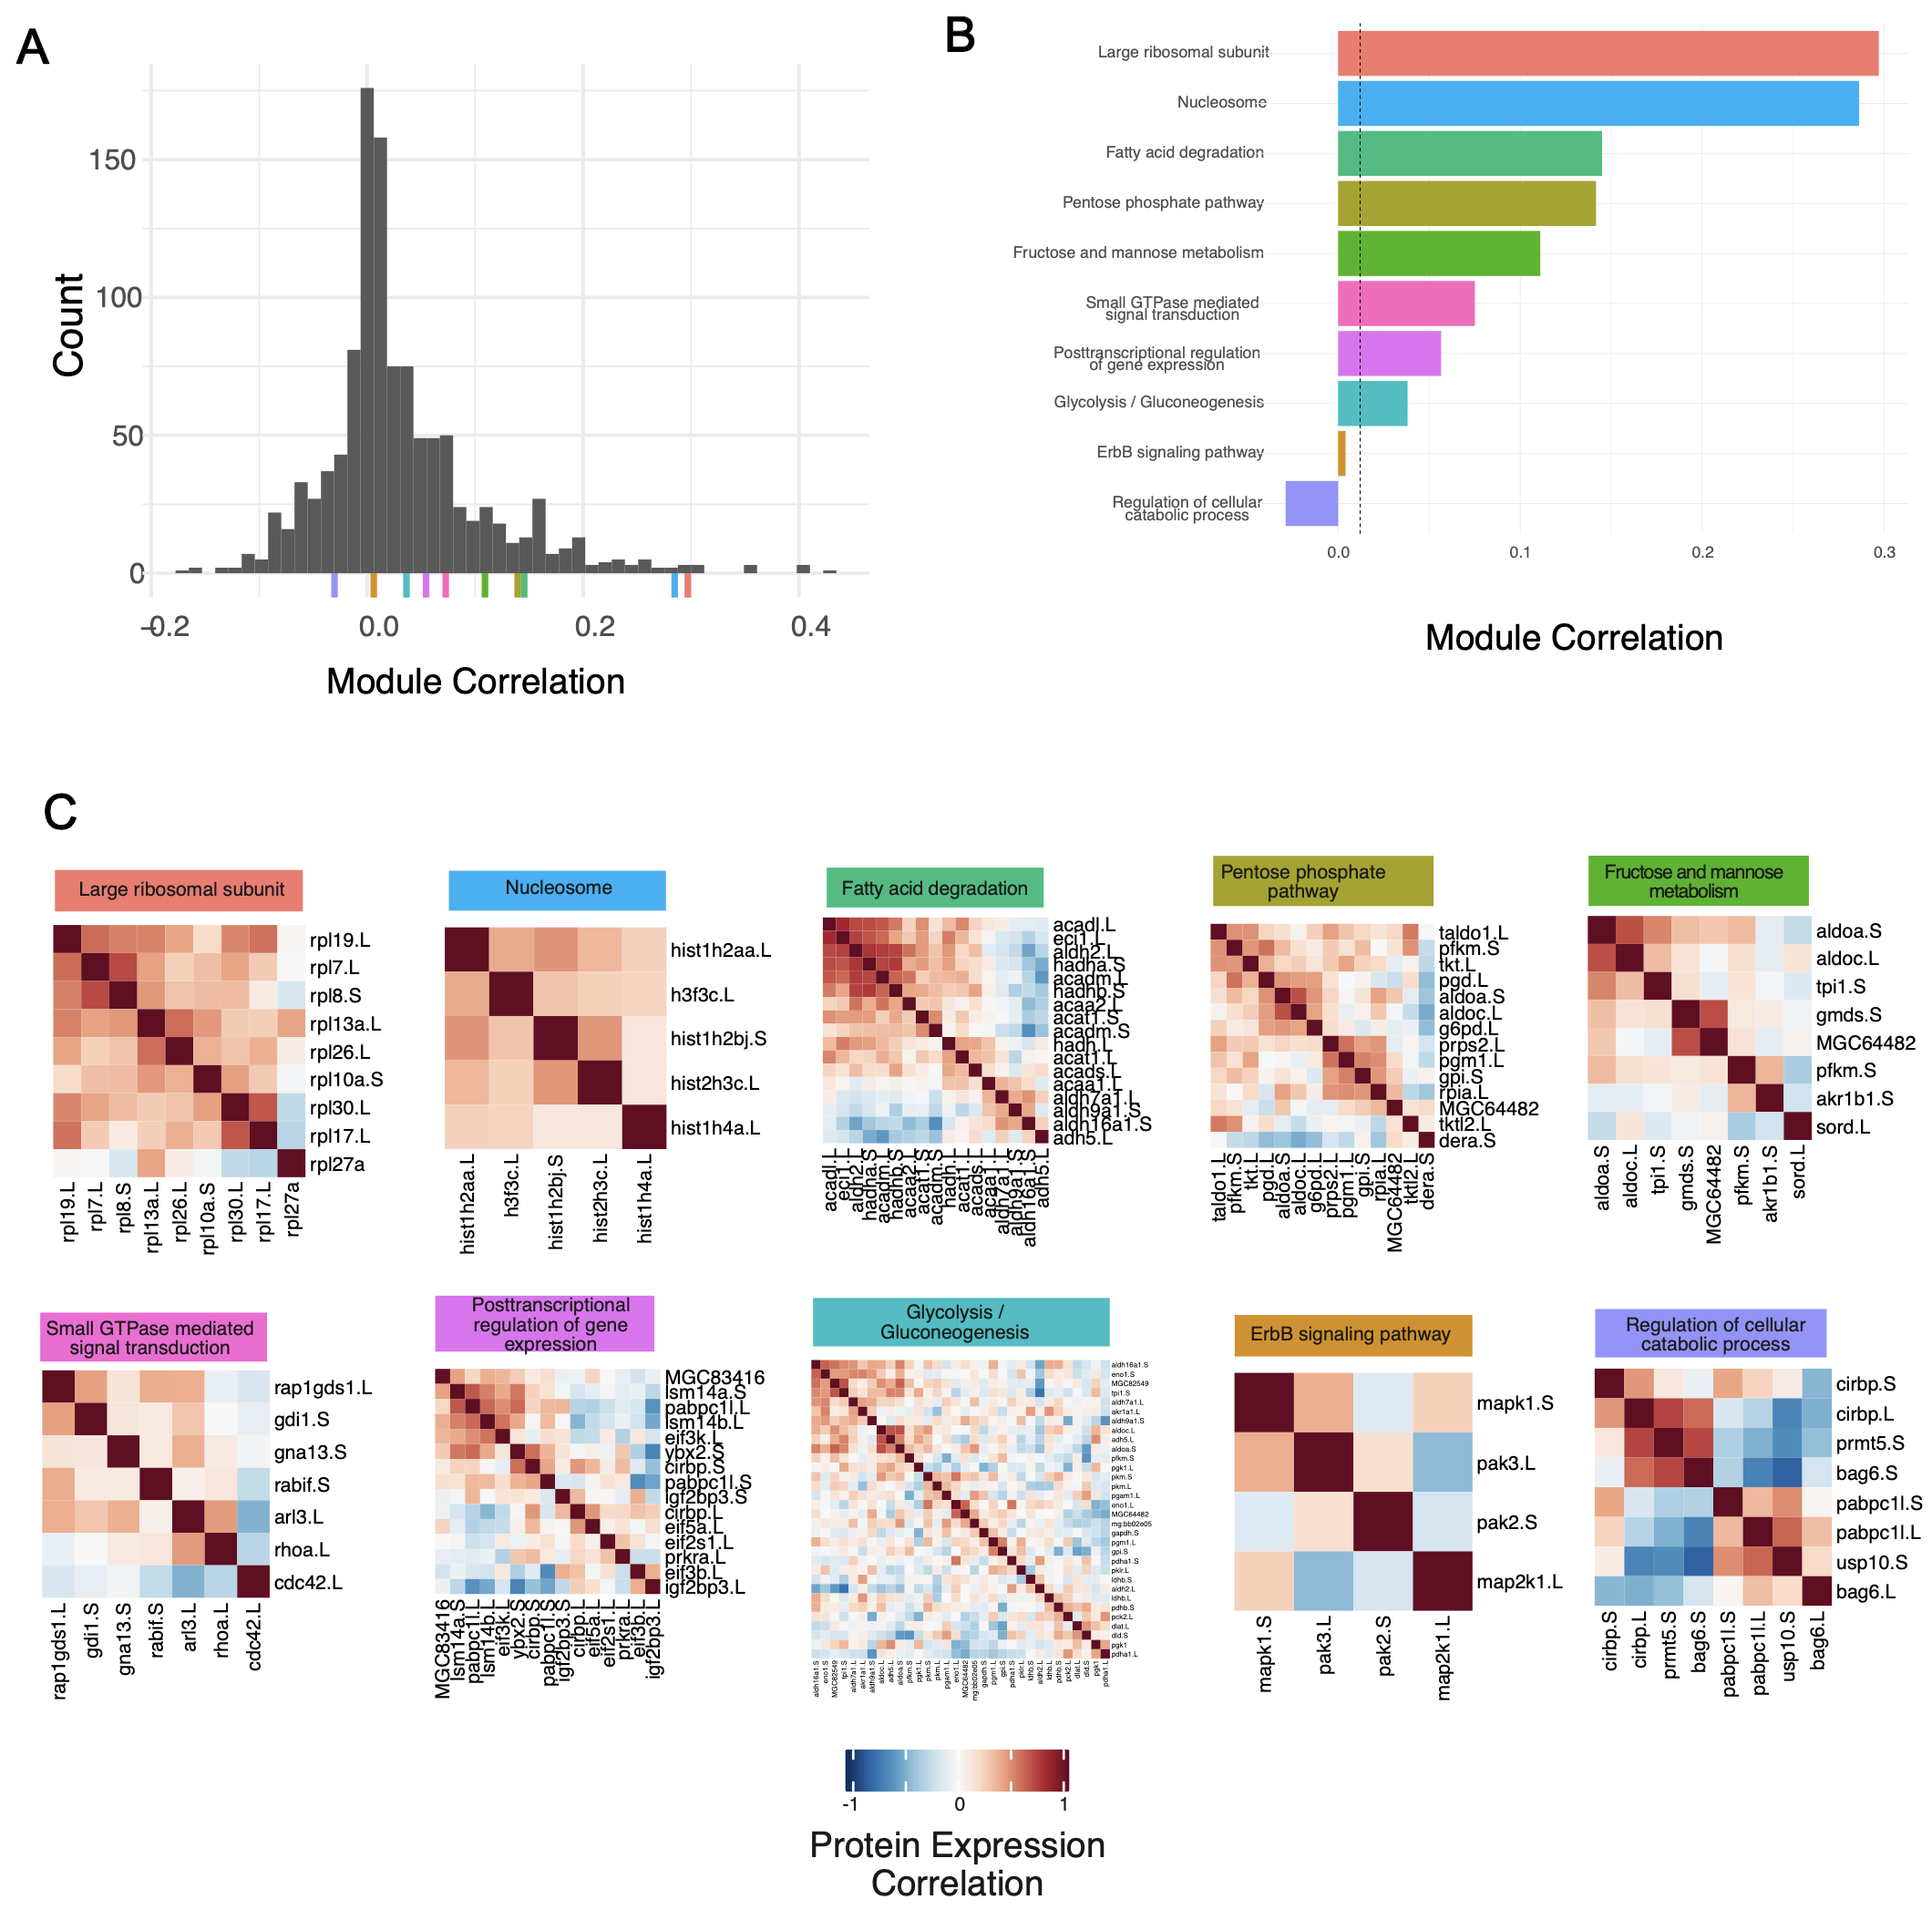
\includegraphics[width=15cm, keepaspectratio]{figs/paper2/fig3.png}
\caption{KEGG pathways and GO Terms can be used to group proteins together to identify modules that on average maintain low and high levels of coordinated expression.}
\caption*{\textbf{(A)} Heat maps of the pairwise correlations between the proteins shown in modules from figure 2. \textbf{(B)} Bar plot of the average of the lower triangular matrix of the module protein expression correlation (module coordinated expression). Dashed line represents the average module coordinated expression of all measured modules in this dataset (1112). \textbf{(C)} Histogram of the average module coordinated expression of all modules analyzed in this dataset (1112). Modules shown in A and B are color coded below the plot.}
\label{fig:paper2_fig3}
\end{figure}

% Figure 4
\begin{figure}[hbt!]
\centering
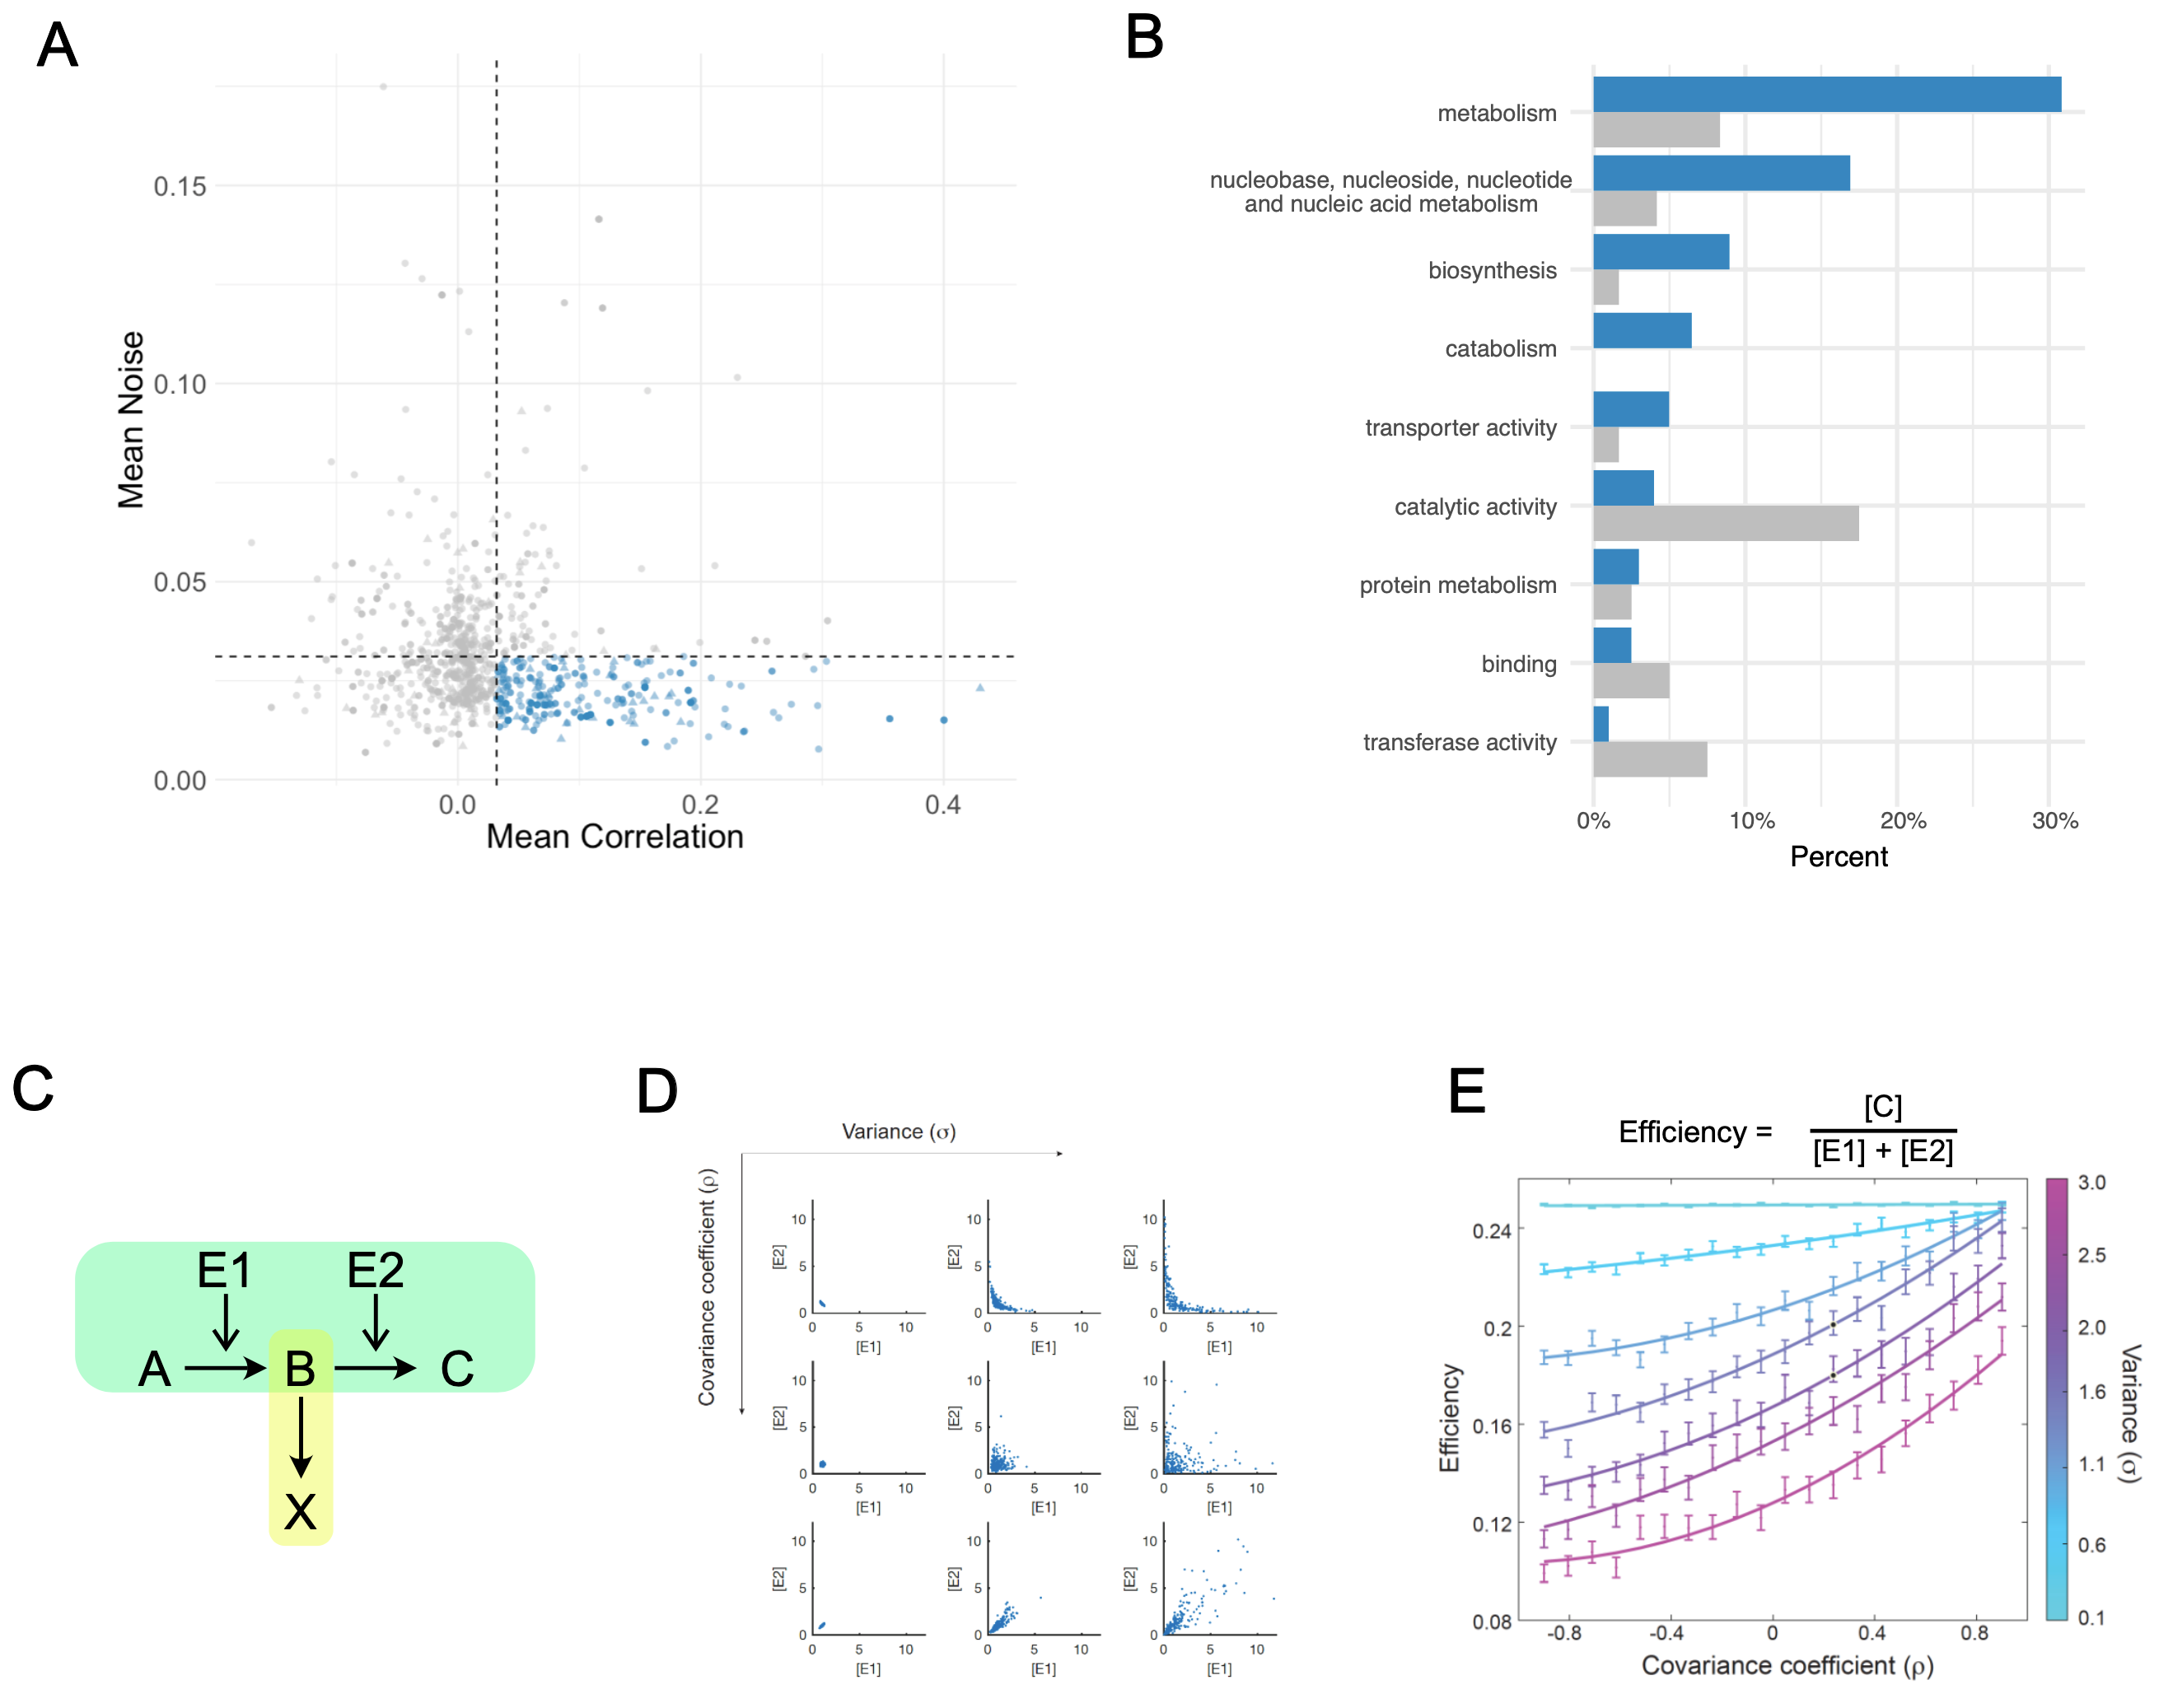
\includegraphics[width=15cm, keepaspectratio]{figs/paper2/fig4.png}
\caption{Metabolic pathways utilize low variance and high correlation of protein expression to increase efficiency.}
\caption*{\textbf{(A)} Pairwise plot between module correlation and module variance. Dashed lines represent the average value of the populations. The low variance and high correlated modules are colored blue. \textbf{(B)} Bar plot of normalized cateGOrizer analysis. The low variance high correlation modules (blue) are compared to the rest of the population (grey). \textbf{(C)} Graphical representation of the metabolic module used to test the effects of variance and correlation on efficiency. The enzymes (E1 and E2) metabolize the substrate (A) into the product (C) via an intermediate molecule (B). This pathway (green) competes for the intermediate with an alternative pathway (X, yellow) for the intermediate molecule. \textbf{(D)} Pairwise plots of enzyme concentrations that were sampled from varying distributions of variance and correlation (1000 cells). \textbf{(E)} Line plot showing the pathway efficiency (y-axis) for varying levels of correlation (x-axis) and variance (color gradient). Points on the graph represent the mean and error bars represent the standard error of the mean.}
\label{fig:paper2_fig4}
\end{figure}

% Figure 5
\begin{figure}[hbt!]
\centering
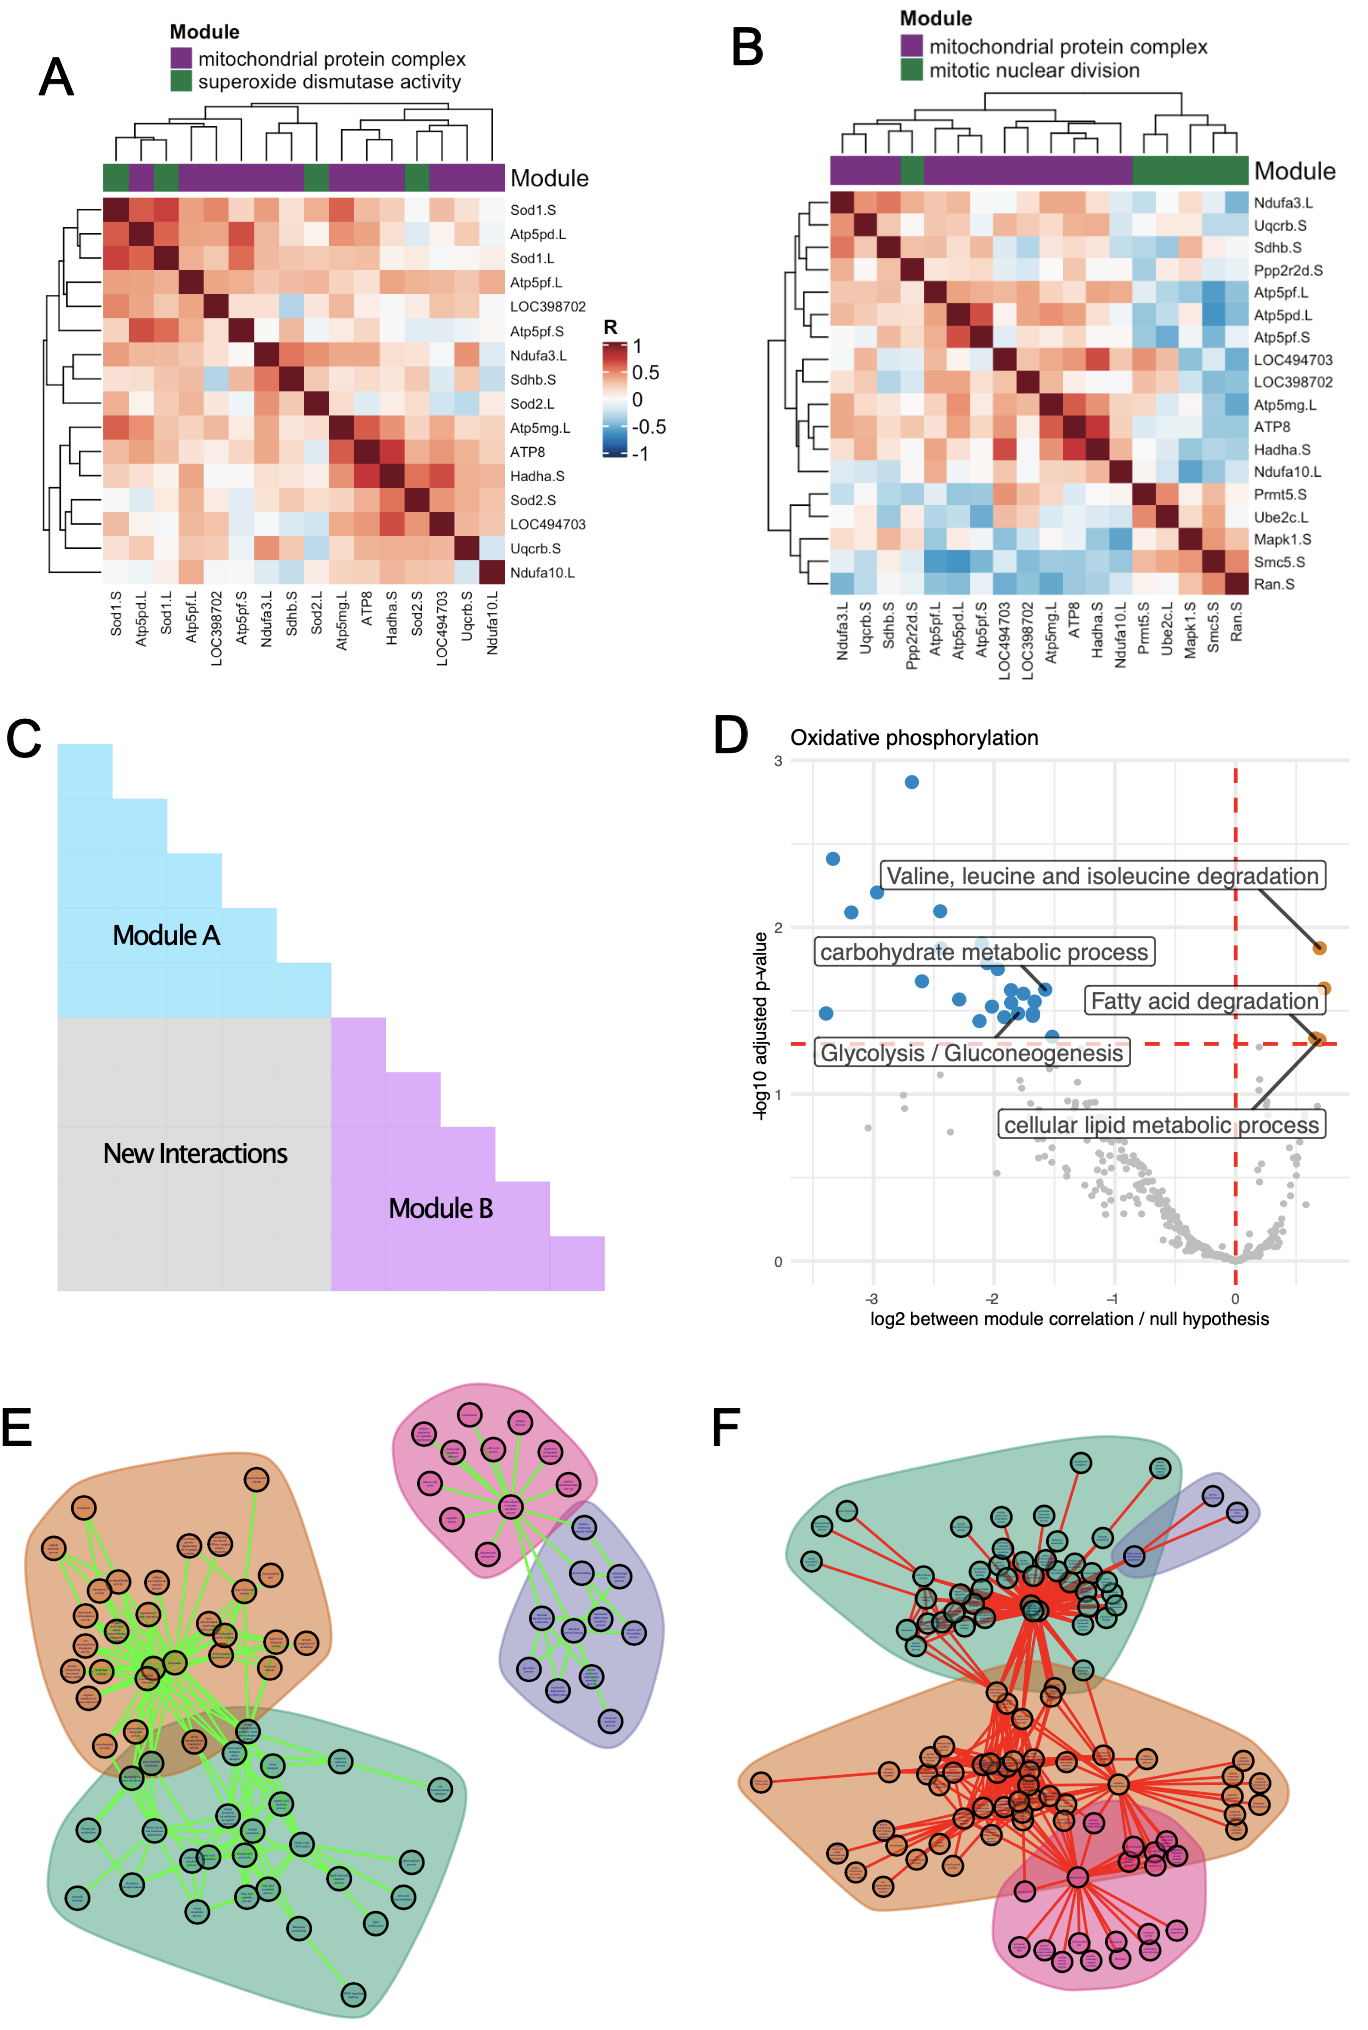
\includegraphics[width=11cm, keepaspectratio]{figs/paper2/fig5.png}
\caption{Bait-prey framework to identify module-module relationships}
\caption*{\textbf{(A)} Clustered heatmap of correlation coefficients between the mitochondrial protein complex and superoxide dismutase activity modules. \textbf{(B)} Clustered heatmap of correlation coefficients between the mitochondrial protein complex and mitotic nuclear division modules. \textbf{(C)} Illustration of between module null hypothesis. All new interactions (grey) between modules A (blue) and B (purple) are assumed to be zero. \textbf{(D)} Volcano plot of log2 transformed ratio of the observed between module correlation value and the calculated null hypothesis (x-axis) and the -log10 transformed FDR corrected p-value. Significant positive modules are colored orange and significant negative modules are colored blue. \textbf{(E)} Network of significant positive modules. \textbf{(F)} Network of significant negative modules.}
\label{fig:paper2_fig5}
\end{figure}
% \include{ch_conclusion}

% uncomment below if you have an appendix
% \appendix
% \chapter{A Long Proof}

\bibliographystyle{unsrt}  % can change to fit your field e.g. pnas2009
\bibliography{mybib}  % no .bib extension necessary

% adds a non-numbered signature page at end (for printing on ACID-FREE paper)
% (remember to comment out when submitting final version)
\onlinesignature

\end{document}
